\documentclass[conference]{IEEEtran}
\IEEEoverridecommandlockouts
% The preceding line is only needed to identify funding in the first footnote. If that is unneeded, please comment it out.

\usepackage{cite}
\usepackage{amsmath,amssymb,amsfonts}
\usepackage{graphicx}
\usepackage{float}
\graphicspath{figures}
\usepackage{listings}
\usepackage{textcomp}
\usepackage{enumitem}
\usepackage{xcolor}
\usepackage{graphicx, float, subcaption}
\usepackage{mathtools}
\usepackage{algorithm}
\usepackage[noend]{algpseudocode}
\usepackage{pifont}
\usepackage{amsthm}
\theoremstyle{definition}
\newtheorem{definition}{Definition}[section]
\theoremstyle{theorem}
\newtheorem{theorem}{Theorem}[section]
\makeatletter
\newenvironment{breakablealgorithm}
  {% \begin{breakablealgorithm}
   \begin{center}
     \refstepcounter{algorithm}% New algorithm
     \hrule height.8pt depth0pt \kern2pt% \@fs@pre for \@fs@ruled
     \renewcommand{\caption}[2][\relax]{% Make a new \caption
       {\raggedright\textbf{\ALG@name~\thealgorithm} ##2\par}%
       \ifx\relax##1\relax % #1 is \relax
         \addcontentsline{loa}{algorithm}{\protect\numberline{\thealgorithm}##2}%
       \else % #1 is not \relax
         \addcontentsline{loa}{algorithm}{\protect\numberline{\thealgorithm}##1}%
       \fi
       \kern2pt\hrule\kern2pt
     }
  }{% \end{breakablealgorithm}
     \kern2pt\hrule\relax% \@fs@post for \@fs@ruled
   \end{center}
  }
\makeatother
\renewcommand{\O}{\,||\,}
\newcommand{\A}{\,\&\&\,}
\usepackage{listings}
%colors
\usepackage{color}
\definecolor{pblue}{rgb}{0.13,0.13,1}
\definecolor{pgreen}{rgb}{0,0.5,0}
\definecolor{pred}{rgb}{0.9,0,0}
\definecolor{pgrey}{rgb}{0.46,0.45,0.48}
\definecolor{light-gray}{gray}{0.95}
\lstset{
	showstringspaces=false,
    breaklines=true,
    backgroundcolor=\color{light-gray},
    tabsize=2,
   	basicstyle=\small\ttfamily,
    %literate={\ \ }{{\ }}1,
    language = Java,
    showspaces=false,
    extendedchars=true, 
    commentstyle=\color{pgreen},
  	keywordstyle=\color{pblue},
  	stringstyle=\color{pred},
  	columns=fullflexible
  	keepspaces=true,
}


\def\BibTeX{{\rm B\kern-.05em{\sc i\kern-.025em b}\kern-.08em
    T\kern-.1667em\lower.7ex\hbox{E}\kern-.125emX}}
\begin{document}

\title{Concurrent Tree Traversals in Binary Search Trees\\
%{\footnotesize \textsuperscript{*}Note: Sub-titles are not captured in Xplore and
%should not be used}
%\thanks{Identify applicable funding agency here. If none, delete this.}
%}
}

\author{\IEEEauthorblockN{Robert Bland}
\IEEEauthorblockA{\textit{College of Engineering and Computer Science} \\
\textit{University of Central Florida}\\
Orlando, FL \\}
\and
\IEEEauthorblockN{Tyler Townsend}
\IEEEauthorblockA{\textit{College of Engineering and Computer Science} \\
\textit{University of Central Florida}\\
Orlando, FL \\}
}

\maketitle

\begin{abstract}
We introduce a reimplementation of a practical and concurrent binary search tree and an AVL tree that uses the PaVT condition, which permits a lock-free contains operation. We utilize this condition by the use of snapshots, which contains a logical ordering of all items in the tree. This is further utilized to determine whether the item exists within the tree based on the ordering. This ordering combined with this condition allows us to construct a lock-free contains to check for any target nodes that have been moved around as a result of another thread's operations.\\
We present a concurrent BST tree that utilizes a lock-free contains, and a concurrent AVL tree that utilizes a lock-free contains that requires the use of atomic snapshots to determine whether the key exists in the data structure. Our insert and remove operation use mutexes to ensure that the snapshots are not mutated by more than one thread at a time and to ensure correctness. \\
We implemented a GCC software transactional memory version of both the concurrent BST and concurrent AVL tree. This is evaluated against our own concurrent implementations to test the effectiveness and performance of the use of transactional memory as well as the performance of our concurrent operations. Our results show that transactional memory has a lower performance than the concurrent data structure.
\end{abstract}

\begin{IEEEkeywords}
Search Trees, Concurrency, AVL, Data Structures
\end{IEEEkeywords}

\section{Introduction}
With the increase in the number of cores on the processor, concurrent datastructures become the foundation to which these cores may be utilized otherwise they become a bottleneck of contention \cite{crain-cont}. Implementing concurrent search trees becomes challenging when modification to the tree can cause relocation of some of the nodes, especially when the trees are optimized for read operations \cite{draschler-pavt}.

The Draschler-Cohen et al. of \cite{draschler-pavt} provide a necessary and sufficient condition for path validation in traversals which they call \textit{PaVT} condition. This condition applies to \textit{any} search tree can validate whether a key is present in the tree or not. They demonstrate that the using the PaVT condition with a Binary Search Tree (BST) and an AVL tree, the out performs existing solutions using a lock-free contains on search-based data structures.

However, evaluating this condition leveraging software transacitonal memeory to manage concurrent accesses has not yet been shown. Concurrent trees using STM are easy to implement and scale well, but STM introduces overhead and where high contention exists still requires some reasearch \cite{bron}. Transactional memory removes the complexity of locks \cite{b4}. Balancing the usefulness of the simple resource sharing and performance is a hard task and the transactional memory implementation emulates just how much has to be sacrificed for reduced complexity. Transactional memory can significantly lower the possibility of data races and deadlocks \cite{b4}.

This paper wishes to show the reimplimentation of the author's BSTs (including AVL) which leverage the PaVT condition. Further extending their work, we implement the BSTs using GCC's software transactional memory (STM) framework and compare the performance of the STM implementation to the BST implementation. The paper will provide a concise background of the PaVT condition presented by the author's work and demonstrate its use in BST's. The implementation details are provided in the following section. Section IV will exam the performance evaluation of all the data structures followed by a brief discussion in section V.
\section{Background}
\subsection{Path Validation Traversal in Search Trees}
\textbf{Pa}th \textbf{V}alidation traversals in search \textbf{T}rees is a necessary and sufficient condition for determining whether a key is existent in any tree. It satisfactory to observe only a limited number of nodes in the path leading to this key defined as the succinct path snapshot (SPS). A path is suitable for a key $k$ if the condition $c_i$ associated with every $node-field$ pair in the path. For a BST the conditions are $C=\{<,>\}$ and field $F=\{L, R\}$. Thus a path from the root, $n_0$, to a an arbitrary node $n_k$ is $P=(n_0, f_0), (n_1, f_1),\cdots, (n_k, f_k)$ where $n_k.f_k = null$ denotes that $n_k$ is the last node in the path as $f_k\not \in F$. The author's formal defintion of the PaVT condition stated in Theorem \ref{thm:pavt}.

\begin{theorem} {(The PaVT Condition)}\label{thm:pavt}
Given a tree $T$ a key k, and a set of node-condition pairs, $S=\{(n_{i_1}, c_{i_1}),\cdots, (n_{i_m}, c_{i_m})\}$, if there exists a moment beteween the traversal's invocation and response where all the following hold:
\begin{enumerate}
\item For every $(n_i, c_i) \in  S, c_i(n_i, k) = 1$
\item $n_{i_1},\cdots, n_{i_m}$ are logically in $T$
\item There is a path in $T$ linking these nodes
\item The path is maximal
\item For every node $n$ logically in $T$, either no node in $S$ is reachable from it or there exists a pair $(n_i, c_i)\in S$ where $n_i$ is reachable from $n$ via a field $f$, and $c_i(n_i, k)$ implies a condition $c(n, k)$ such that $c \implies f$ is the next field.
\end{enumerate}
Then there is no node logically in $T$ with a key $k$.
\end{theorem}

Applying this to a BST, if there is a path $P=(10,L),(8,L),(3,R),(4,R)$, then the suitable keys for this path are $k\in\{5, 6, 7\}$. If this path was taken to search for key $k=9$, then some mutation must have occured and the traversal would need to restart.   

\subsection{Succinct Path Snapshot}
Maintaing a full path is difficult as part of the path may have an inconsistency from some other mutation. Therefore, the authors formally define a succinct path snapshot which decouples 1) from the PaVT, and allows for concurrent mutations to change nodes that link the snapshots, but do not affect the snapshot. There is a transitivity property for the paths as we traverse them. For example $P=(10,L),(8,L),(3,R),(4,R)$  can be reduced to $P=(8,L),(4,R)$ since $5>4 \implies 5 > 3$  and $5<8 \implies 5<10$. This would be the maximal set of nodes with respect to all the conditions for a BST i.e, $(<,L), (>, R)$. This is known as the \textit{succinct path snapshot} (SPS). The author's formal definition is stated below.
\theoremstyle{definition}
\begin{definition}{(Succinct Path Snapshot)} Let $P = (n_0, f_0),\cdots,(n_m, f_m)$ be a path and $C'=(n'_0, c_0),\cdots (n'_k, c_k)$ be a node-condition series corresponding to $P.S\subseteq C$ is a succinct path snapshot (SPS) of P if:
\begin{enumerate}
	\item $n'_0\cdots, n'_k$ are logically in $T$
	\item There is a path in $T$ linking these nodes which is maximal if $n'_k.f_k = null$
	\item For every node $n$ logically in $T$, either no node in $S$ is reachable from it, or there exists a pair $(n_i, c_i) \in S$ where $n_i$ is reachable from $n$ via some field $f$ such that for every $k$, $c_i(n_i, k)$ implies $c(n, k)$ that returns $f$ for all valid keys $w.r.t$ $S$ of $n$.
	\item For every $(n_i, c_i), (n_j, c_j) \in S$ such that $j > i$ and for every key $k$, $c_j(n_j, k)$ does not imply $c_i(n_i, k)$ for some valid key w.r.t. $S$ of $n_i$.
\end{enumerate}
\end{definition}
The validation of an SPS is not only sufficient but necessary for unsuccessful traversals. The author's state that for BST's, the snapshots can be optimized by observing that for any node $n$, that $n$'s left snapshot $S_L$, and $n$' right snapshot $R_L$ consist of its predecessor and successor, respectively,  in the logical ordering of the tree \cite{draschler-lo}. Our implementation uses pointers to maintain a reference to the predecessor and successor for a node. In order to ensure that all node's snapshots are of the same size, sentinel nodes are used to maintain order.

\subsection{Correctness}
Correctness of maintaining snapshots follows from the fact that if an update to a path is occuring, all locks must be acquired before the operation. Therefore, the snapshots are guaranteed to reflect those of the path. 
\subsection{Linearizability}
Snapshots are read and written to atomically which allows them to be linearized. The linearization point for a snapshot is the moment it is an SPS of a path in the tree. These snapshots can be linearized with respect to the operations. If the snapshot were to contain a node that has been removed, it is linearized just prior to the removal. If the snapshot does not contain a node that is now reachable via an insertion, it is linearized just before it was added. The idea is that if the snapshot has been read, then it is from a path that existed in the tree, and the fact that it is read means that the operating thread performing a mutation has not completed it's operation. 
\section{Data Structure Design Principles}

The author's paper presented the topic of \textit{PaVT} and provided little detail on the implementation of the data structure. Available pseudocode was used to construct the methods necessary for the BST data structure. Since only a brief description of the AVL rebalancing property was mentioned, an attempt to construct the AVL function was taken. We contacted the author's about some synchronization issues not explicitly stated in the paper, particularly about updating snapshots. As of Nov. 8, 2018, the source code for the author's implementation is available at {https://github.com/logicalordering/trees}. We borrowed the synchronization for snapshots, particuarly, for removal from their source code. Thus our source code is an amalgam of their pseudo and source code. In the following subsections, we will discuss the design of our implementation, including the main algorithms.

\subsection{Tree Structure}
Our tree structure implements both the Binary Search Tree ordering property, but provides a boolean argument to the constructor to specify the AVL structure property. The AVL operation \textbf{rebalance} is performed at the end of the \textbf{insert} and \textbf{remove} operations of the tree. This allowed the code to follow the \textit{DRY} principle. The remaining functions \textbf{traverse} and \textbf{contains} are almost identical except that \textbf{traverse} will lock the node to be returned while \textbf{contains} returns a boolean value.

The tree has four member variables; three of \textit{Node} and the fourth is the \textit{AVL} boolean. The \textit{Node} class can be seen in Figure \ref{fig:node}. The key values are represented as integers for simplifying the data structure requirements. In order for the structure to meet the correctness requirements, the Node class must allow the node to be marked. This will depict a logical removal when $n.mark = true$. This is done right before a node becomes unreachable. The keys are immutable, so nodes cannot be recycled. This prevents nodes from needing to be rechecked. If a node is logically in the tree, it is reachable. 

We store the snapshots of the node as atomic pointers. This allows the snapshots to be linearized when they are read. Each node also a parent pointer as well as left and right pointers to its children, which allows traversing up the tree. A height field is provided to store the current height of the tree. A tree with no node has height $-1$, a single node, 0, and the height of the tree is the maximum of the left, and right subtrees + 1.

The tree has four member variables; three of \textit{Node} and the fourth is the \textit{AVL} boolean. Two of the three pointers are sentinel nodes. The sentinel nodes are represented as the maximum and minimum, signed 32-bit integers in C. This does give some restriction on the number of keys to use, but this was done as the testing environment would only handle a maximum of 5,000,000 nodes. The snapshots of the sentinel nodes contained each other. The minimum sentinel was the parent of the max sentinel and the max sentinel was also the root of the tree, the third pointer.
\begin{figure}[t]
\label{fig:node}
\centering
\begin{lstlisting}
class Node {
	const int data;
	bool mark;
	std::mutex lock;
	std::atomic<Node *> leftSnap;
	std::atomic<Node *> rightSnap;
	Node *left;
	Node *right;
	Node *parent;
	int height;
}
\end{lstlisting}
\caption{The Node data structure implemented within the BinarySearchTree class}.
\end{figure}

\subsection{Locking Protocol}
The locking order of the lock's is such that if $n_1$ and $n_2$ are nodes in the tree, then $n_1$'s lock is acquired before $n_2$'s lock if: (1) $n_2$ is reachable from $n_1$, (2) $n_1$ and $n_2$ are reachable by a field $f_i$ and $f_j$, respectively from their lowest common ancestor and $i<j$. This is an essential top-down, left-to-right locking order. The implementation of the data structure; however, will lock the node to be removed, $n$, prior to locking the parent's node, $p$. In this case, an optimistic attempt will be taken to acquire the lock. If it fails, then both lock's are realeased and the operation is reattempted.

This protocol is livelock and deadlock free since locks are acquired in the same order by all threads. At least one thread can make progress since the lowest node in the tree (level-ordering) is guaranteed to acquire all necessary locks.

\subsection{Traverse/Contains}
Algorithm \ref{alg:contains} starts from the root of the tree and uses a helper function \textbf{nextField} to reach the next node. If the node is the last in the path, \texttt{nextField} will be such that if $f=\mathbf{nextField}(n, key)$ then $n.f = null$. If the node with $key$ is found then the function returns true if the node is not marked. If it is the function restarts. For \textbf{traverse} the node is locked just before line \ref{alg:contains:lock}. Since the thread waits for the lock, we check if the node has been marked for deletion. If so, the node is unlocked and the procedure is restarted. If the end of the path is reached, the last node in the path is locked and snapshot for the node and field is read atomically. If the key is not in the node's snapshot, the procedure is restarted otherwise the node is returned. And for \textbf{contains}, the function simply returns false.

Being read atomically allows the snapshot to be linearized when either (i) the unmarked node with the key is found or (ii) the linearization point of the snapshot read at line \ref{alg:contains:snap}. For (i) since the node was found and locked, this node is currently reachable in the tree. The read snapshot from (ii) guarantees  that this snapshot captures the suitable path for the key. If it has not, then a mutation has occurred to alter the path such that the current thread would have traversed to the current node which indicates the procedure to restart.
%\begin{algorithm}[H]
%\caption{Traverse (node, key)}
%\label{alg:traverse}
%\begin{algorithmic}[1]
%\State $n\gets node$
%\State $f \gets \mathbf{nextField}(n, key)$
%\State $next \gets n.f$
%\While {$next \neq null$}
%  \State $n\gets next$
%  \State $f \gets \mathbf{nextField}(n, key)$
%  \If {$n.k = key$}
%  	\State $lock(n)$
%  	\If {$n.mark = true$}
%  		\State $unlock(n))$ \textbf{then} restart
%  	\EndIf
%  	\State \Return $n$
%	\EndIf
%	\State $next \gets n.field$
%\EndWhile
%\State $S \gets (field = L$ ? $n.S_L$ : $n.S_R)$ \label{alg:traverse:snap}
%\If{($f = L$ \textbf{and} $key \not \in (S, n)$) \textbf{or} ($f = R$ \textbf{and} $key \not \in (n, S))$}
%\State $unlock(n))$ \textbf{then} restart
%\EndIf
%\State \Return $n$
%\end{algorithmic}
%\end{algorithm}

\begin{algorithm}[t]
\caption{Contains (key)}
\label{alg:contains}
\begin{algorithmic}[1]
\State $n\gets root$
\State $f \gets \mathbf{nextField}(n, key)$
\State $next \gets n.f$
\While {$next \neq null$}
  \State $n\gets next$
  \State $f \gets \mathbf{nextField}(curr, key)$
  \If {$n.k = key$}
  	\If {$n.mark = true$} \label{alg:contains:lock}
  		\State restart
  	\EndIf
  	\State \Return true
	\EndIf
	\State $next \gets n.field$
\EndWhile
\State $S \gets (field = L$ ? $n.S_L$ : $n.S_R)$
\If{($f = L$ \textbf{and} $key \not \in (S, n)$) \\ \textbf{or} ($f = R$ \textbf{and} $key \not \in (n, S))$} \label{alg:contains:snap}
\State restart
\EndIf
\State \Return false
\end{algorithmic}
\end{algorithm}

\subsection{Insert}
Algorithm \ref{alg:insert} begins by calling \textbf{traverse} starting at the root for $key$. If the node returned, $n$, has a key equal to $key$ or the node is no longer the end of the path (i.e., another insertion has occurred on the same node) then the procedure is restarted. Otherwise a new node $newNode$ is allocated with its parent pointer set to $n$. Snapshots are updated based on the value of the $key$. The snapshot for $n$ and $n$'s snapshot, $S$ must be updated so that $newNode$ is contained in their snapshots while $newNode's$ snapshots consists of both $n$ and $S$. This is done prior to making $newNode$ reachable from $n$ which is the moment of linearization. 
\begin{algorithm}[t]
\caption{Insert (key)}
\label{alg:insert}
\begin{algorithmic}[1]
\State $n\gets \mathbf{traverse}(root, key)$
\If {$n.k = key$ \textbf{or} ($key>n.k$ \textbf{and} $n.R \neq null$) \textbf{or} ($key<n.k$ \textbf{and} $n.L \neq null$)}
	\State $unlock(n)$ \textbf{then} restart
\EndIf

\State $newNode\gets \mathbf{new} Node(key)$
\State $newNode.P \gets n$
\State $S \gets (n.k > newNode.k$ ? $n.S_L$ : $n.S_R$
\If {$n.k > newNode.k$}\label{alg:insert:snaps}
	\State $newNode.S_L \gets S$
	\State $newNode.S_R \gets n$
	\State $S.S_R \gets newNode$
	\State $n.S_L \gets newNode$
	\State $n.L \gets newNode$
\Else
	\State $newNode.S_L \gets n$
	\State $newNode.S_R \gets S$
	\State $S.S_L \gets newNode$
	\State $n.S_R \gets newNode$
	\State $n.R \gets newNode$
\EndIf
\State $unlock(n)$
\If {$AVL$} $\mathbf{rebalance}(n)$
\EndIf
\end{algorithmic}
\end{algorithm}

\subsection{Remove}
Algorithm \ref{alg:remove} traverses to the node to be removed. If $n.k\neq key$, then by the PaVT condition, the tree does not contain $key$ and it returns. Otherwise, an optimistic attempt to lock the parent is taken. If it fails, the procedure restarts. Once both are locked, the possible scenarios are:
\begin{enumerate}
\item $n$ is a leaf
\item $n$ has one child, $c$
\item $n$'s right child, $r$, does not have a left subtree
\item $r$ has a left subtree which contains $n$'s successor $s$
\end{enumerate}
The first case is simple as all locks are acquired. The node is marked and the snapshots are updated, $S_{max}$, and $S_{min}$. The corresponding snapshot and $p$ snaps are updated to contain each other as seen starting at line \ref{alg:remove:leaf}. If $n$ has one child, then $c$ takes $n$'s place. Now $n$'s snapshots will be updated to contain each other at line \ref{alg:remove:child}. If the node has 2 children, but $r.L = null$, then $r$ is $n$'s successor and $r$ takes $n$'s place. The most difficult remove is derived when $s$ is in $r$'s left subtree. However, since $r$ has a reference to it, locking the node is done directly along with $s$'s parent $p_s$, its right child, $r_s$, and $s$'s right snapshot $(S_R)_s$. These are locked using the locking order. It is important to check conditions such that $s.P \neq r$ since $r$'s lock is acquired. If this is carried out then the thread will block itself. After acquiring all the locks, the removal can take place and the snapshots are updated at line \ref{alg:remove:hard:snap}. Snapshots during a remove require the left and right snapshots of $n$ to update such that $S_L.S_R = S_R.S_L$. This removes $n$ from the logical ordering. $AVL$ rebalancing is performed at the end of the algorithm if necessary. Since the algorithm only proceeds once all locks are acquired, $remove$ is linearized when the node is marked. If \textbf{contains} returns true on $n$, then the node has not been marked. If the node is found marked, then the operation simply restarts.
\begin{algorithm}[th]
\caption{Remove (key)}
\label{alg:remove}
\begin{algorithmic}[1]
\State $n\gets \mathbf{traverse}(root, key)$
\If {$n.k \neq key$} $unlock(n);$ \Return
\EndIf
\State $p \gets n.P;\,l\gets n.L;\, r\gets n.R$
\If {!$tryLock(p)$} $unlockAll()$ \textbf{then} restart
\EndIf

\If {$n$ is a leaf}
	\State $S_{\max} \gets n.S_R;\, S_{\min} \gets n.S_L$
	\State $n.mark\gets true$
	\If {$p.k > n.k$}\label{alg:remove:leaf}
		\State $p.L \gets null;\,p.S_L \gets S_{\min};\, S_{\min}.S_R \gets p$
	\Else
		\State $p.R \gets null;\,p.S_R \gets S_{\max};\, S_{\max}.S_L \gets p$
	\EndIf
	\State $unlockALl()$
	\If {$AVL$} $\mathbf{rebalance}(p)$; \Return
	\EndIf 
\EndIf

\If {$n$ has one child}
	\State $\alpha \gets l=null;\, c\gets (\alpha$ ? $r$ : $l$)
	\State $S_{\max} \gets n.S_R;\,S_{\min} \gets n.S_L$
	\State $snap \gets (\alpha$ ? $S_{\max}$ : $S_{\min})$
	\State $lock(c, snap)$
	\If {($\alpha \A snap.S_L \neq n) \O (!\alpha \A snap.S_R \neq n$)}
		\State $unlockAll()$ \textbf{then} restart
	\EndIf
	\State $n.mark\gets true$
	\State $(p.L = n$ ? $p.L$ : $p.R) \gets c$
	\State $S_{\min}.S_R \gets S_{\max};\,S_{\max}.S_L \gets S_{\min}$ \label{alg:remove:child}
	\State $unlockALl()$
	\If {$AVL$} $\mathbf{rebalance}(p)$
	\EndIf
	\Return
\EndIf

\State $l \gets n.L;\,r\gets n.R;\,S_{\min} \gets n.S_L;\,S_{\max} \gets n.S_R$
\State $lock(l, r, S_{\min}, S_{\max})$
\If {$S_{\min}.S_R \neq l\,||\, S_{\min}.mark$}
	\State $unlockAll()$ \textbf{then} restart
\EndIf

\If{$r.L = null$}
	\State $n.mark \gets true$
	\State $r.L \gets l;\,l.P \gets r;\,r.P\gets p$
	\State $(p.L=n $ ? $p.L$ : $p.R) \gets r$
	\State $S_{\min}.S_R \gets S_{\max};\,S_{\max}.S_L \gets S_{\min}$
	\State $unlockALl()$
	\If {$AVL$} $\mathbf{rebalance}(r)$
	\EndIf
	\Return
\EndIf

\State $s\gets S_{\max};\,p_s \gets s.P; \,r_s \gets s.R;\,({S_R})_s \gets s.S_R$
\State $lock(s, p_s, r_s, ({S_R})_s)$
\If {$s.S_L \neq n \,||\, s.mark || ({S_R})_s.S_L \neq s || ({S_R})_s.mark$}
	\State $unlockAll()$ \textbf{then} restart
\EndIf

\State $n.mark\gets true$
\State $s.R\gets r;\, r.P \gets s;\, s.L\gets l;\, l.P \gets s$
\State $(p.L=n $ ? $p.L$ : $p.R) \gets s$
\State $p_s.L\gets r_s$
\If {$r_s\neq null$} $r_s\gets r_s$
\EndIf
\State $S_{\min}.S_R \gets S_{\max};\,S_{\max}.S_L \gets S_{\min}$ \label{alg:remove:hard:snap}
\State $unlockALl()$
\If {$AVL$} 
\State $\mathbf{rebalance}(s);\,\mathbf{rebalance}(p_s)$
\EndIf
\end{algorithmic}
\end{algorithm}

\subsection{Rebalance}
The \textbf{rebalance} operation is implemented based on the author's description \cite{pavt}. This algorithm starts at the specified node, $n$ and traversed to the root. It grabs it's parent, $p$, and lock's both in the described locking order. If now calculates the node's height, $h'$, and check if its member variable height, $n.h$ is different. If so, there has been a mutation, and the new height is updated. The balance factor is calculated $bf$, which is the difference between the left and right subtrees. If the height has not changed and $|bf|<2$, then we return which is our implementation of the relaxed rebalancing. Rather than traversing entirely to the root. If $bf\geq 2$, then we must rotate. Helper functions \textbf{rotateLeft()} and \textbf{rotateRight} are implemented to carry this out. If $bf<-1$ and the left child of $n$ has a positive balance factor, then a double rotation is required, and conversely for $bf>1$. The nodes necessary for this operation will be the child and its grandchild. Locks are acquired from parent to grandchild. Since the rotations will now reorder the nodes, the locking order changes when they are released. The code is implemented in a straight forward manner to illustrate this. However, rotations for $m$-arry trees perserve the logical ordering which in turn preserves the snapshots, hence they will not need to be updated. If an insert or remove is interacting with this operation, the linearization point of this occurs once all the locks are released for every traversal up the tree. For a contains, the linearization point occurs during the last rotation. Any incorrect traversal will be reflected by the snapshots.
%
%\begin{breakablealgorithm}
%\caption{Rebalance (node)}
%\label{alg:rebalance}
%\begin{algorithmic}[1]
%\State $p\gets n.P$
%\While {$n\neq root$}
%	\State $lock(p)$
%	\If{$n.P\neq p$}
%		\State $unlock(p)$
%		\If {$n.mark=true$} \Return
%		\EndIf
%	\EndIf
%	\State $lock(n)$
%	\If {$n.mark=true$} 
%		\State $unlockAll()$
%		\Return
%	\EndIf
%	\State $h' \gets \mathbf{height}(n)$
%	\State $bf \gets \mathbf{height}(n.L) - \mathbf{height}(n.R)$
%	\If {$h'\neq n.h$}
%		\State $n.h \gets h'$
%	\ElsIf {$bf \leq 1$}
%		\State $unlockAll()$ \textbf{then }\Return
%	\EndIf
%	\If {$bf>1$}
%		\State $c\gets n.R;\,g_c \gets c.L$
%		\State $lock(c)$
%		\State $bf_c \gets \mathbf{height}(c.L) - \mathbf{height}(c.R)$
%		\If{$bf_c < 0$}
%			\State $lock(g_c)$
%			\State \textbf{rotateRight}$(g_c, c, n$)
%			\State \textbf{rotateLeft}$(g_c, n, p$)
%			\State $unlockAll()$
%			\State $n\gets g_c$
%		\Else
%			\State \textbf{rotateLeft}$(c, n, p$)
%			\State $unlockAll()$
%			\State $n\gets c$
%		\EndIf
%	\ElsIf{$bf<-1$}
%		\State $c\gets n.L;\,g_c \gets c.R$
%		\State $lock(c)$
%		\State $bf_c \gets \mathbf{height}(c.L) - \mathbf{height}(c.R)$
%		\If{$bf_c > 0$}
%			\State $lock(g_c)$
%			\State \textbf{rotateLeft}$(g_c, c, n$)
%			\State \textbf{rotateRight}$(g_c, n, p$)
%			\State $unlockAll()$
%			\State $n\gets g_c$
%		\Else
%			\State \textbf{rotateRight}$(c, n, p$)
%			\State $unlockAll()$
%			\State $n\gets c$
%		\EndIf
%	\Else
%		\State $unlockAll()$
%		\State $n\gets p$
%		\State $p\gets n.P$
%	\EndIf
%\EndWhile
%\end{algorithmic}
%\end{breakablealgorithm}

\subsection{STM Implementation}
\begin{figure*}[t]
 \centering
\begin{minipage}{0.49\textwidth}
\begin{lstlisting}
void insert(int const &data){

  while (true) {
  
    __transaction_atomic{
    	n = traverse(root, data)
      /* Do insert op */
      if (isAvl) rebalance(n);
    }
  }
}  
\end{lstlisting}
\textbf{(a) Initial Implementation. Entire function is encapsulated in atomic block.}
\end{minipage}
\begin{minipage}{0.49\textwidth}
{\begin{lstlisting}
void insert(int const &data){

  while (true) {
    n = traverse(root, data)
    __transaction_atomic{
			/* Check snapshots */
      /* Do insert op */
    }
   	if (isAvl) rebalance(n);
  }
}  
\end{lstlisting}
}
\textbf{(b) Second Implementation. Traverse and Rebalance function are decoupled from write operations.}
\end{minipage}
\caption{Implementing the atomic\_transaction block in the data structure}
\end{figure*}

\subsubsection{GCC Transactional Memory}
GCC's STM framework is used for the STM BST implementation. GCC transactional memory is used to create blocks of code that will be executed atomically. If another transaction block (or thread) causes a conflict on a memory access with the current block then we abort and rollback all modifications and try the transaction. This transactional memory also has specific properties associated with it as well that can be applied to any variable or function. The two properties are defined as transaction safe and transaction unsafe. For the transaction unsafe property, it is assumed if the code has or contains the following \cite{b4}:
\begin{itemize}
\item it is relaxed transaction statement (we don't use this)
\item it contains an initialization of, assignment to, or a read from a volatile object
\item it is unsafe asm declaration
\item it contains a function call to a transaction-unsafe function, or through a function pointer that is no transaction-safe
\item it has a volatile variable (so no atomic or volatile variables)
\end{itemize}

The transaction safe property, however, will be allowed to execute inside the atomic block of code if it isn't declared transaction unsafe. There are even more rules to what is exactly transaction safe and unsafe, but that is very complicated and some irrelevant, so a reference is provided for knowing more about this \cite{b4}. 

\subsubsection{Implementation Breakdown}

then modifying it by surrounding code that will be shared or expected to be modified by other threads in a transaction atomic block. The sequential version of the GCC transactional memory implementation used this style, but in a very broad sense. The sequential implementation involved the removal of all atomic wrappings, so no atomic variables, and the removal of all mutexes, so removing all locks and unlock calls from the code as well. These two actions plus inserting a transactional block of code for all of our function lead to the following sequential implementation for insert:

Implementing the most basic form of transactional memory was simple and straight forward, but increasing the performance was tricky. so that the transactions are smaller. It is implemented such that the transactions are light weight to ensure that when a transaction does fail it won't have to retry more code than it has to. The improvements made to the original implementation was removing transactions from contains and traverse since they do no write operations. Another change made was to decouple the traverse from the insert and remove. This small change made it, so the implementation doesn't have to retraverse the tree. Some checks have been inserted as a result to ensure that the current node that is being worked on is still a valid option. Another modification made to increase performance was the decoupling of rebalance from insert and remove to increase performance of AVL tree operations. Before it would


\section{Performance Evaluation}
Testing the implementation was done on Intel(R) Core(TM) i5-4460 CPU @ 3.2GHz with: Max Memory Bandwidth 25.6 GB/s, Number of Cores 4, Number of Threads 4, 6 MB SmartCache, 24.0 GB RAM, 64 - bit Windows OS, Run through Ubuntu terminal shell for Windows. It should be noted that the performance is expected to significantly decrease across all platforms when the number of threads increase past four because of hardware limitations. The concurrent data structure is expected to do significantly better than the software and improved software data structure because of how transactional memory operates. The number of benchmarks was three and those three were:
\begin{itemize}
\item 9\% Insert, 1\% Remove, 90\% contains
\item 20\% Insert, 10\% Remove, 70\% contains
\item 50\% Insert, 50\% Remove, 0\% contains
\end{itemize}
This was carried out by providing 5,000,000 operations for the threads to perform, overall. Each tree was populated to its expected capacity. That is for test 1, the tree would be at 90\% expected capacity or 450,000 nodes, 2/3 capacity, and 50\% capacity, respectively for the last two.

\subsection{Concurrent Data Structure}
The results for the lock-based concurrent data structure can be seen in Figure \ref{fig:data}. The AVL tree outperforms BST in most scenarios due to the $O(n\lg n)$ traversals from rebalancing. Where the performance decreases is when rebalancing will get called more often and cause threads to lock nodes that other threads require. Another possible reason why the performance starts to equalize around 50\% contains and removes is because of how costly it is to remove non-leaf nodes. Any leaf node will require at most two locks, while removals of non-leaf nodes could require up to nine. In BST's, the removal and insertion have a much higher chance of creating leaf nodes. The number of leaf nodes in AVL tree is significantly lower due to rebalancing. In fact the upper bound for a balanced BST is $O(n/2)$ leaf nodes. The performance for 50\% inserts and removes demonstrates that with a rebalancing operation performance is not particuarly enhanced. With a 90\% contains ratio, the AVL tree can handle up to 10 MOps/sec.

\subsection{Software Transactional Memory Data Structure}
Our software transactional memory data structure performance is shown by Figure \ref{fig:data}. The performance of AVL is higher than BST in all scenarios with the exception of the 50\% removes and inserts scenario. This is due to the costly nature of rebalancing in AVL, which allowed BST to be on equal terms when using 1 or 2 threads. The performance in all three graphs are significantly lowered when moving from 4 to 8 threads. The reason being for this is that the hardware has limited how well the threads can process these atomic transaction. This hardware limitation increases the chance of a transaction not completing because a single processor starting two different transactions will cause one of them to stall. Furthermore, if both transactions have any conflicts and one finishes then it will cause the other to fail and restart. This leads into a massive increase in failed atomic transactions and is the reason for this decline in the graph. A reason for AVL outperforming BST in most scenarios is due to the fast traverse and contains operations since the graph is more balanced as shown by (b) and (e) in Figure \ref{fig:data}. Traverse and contains are both faster in AVL trees because having fewer leaf nodes and a more compact tree, which is due to rebalancing, means threads won't have to go far to find their target.
\subsection{Improved Software Transactional Memory Data Structure}
In the results shown for our improved software transactional memory in Figure \ref{fig:data}, BST has overtaken AVL in most scenarios, where the only exception being 1 or 2 threads being used in Figure \ref{fig:data} (c). The reason for this is because of decoupling traverse from the atomic transaction block. This allowed for how insert and remove transactions to not restart completely or don't restart while traversing. AVL and BST perform worse in both STM and Modified STM implementations because changing snapshots will cause transactions to restart since snapshots are updated in both insert and remove. Decoupling traverse is one reason why the performance for 8 threads for BST in Figure \ref{fig:data} (c) can do about 3.5 million more operations per second than in (f). Decoupling rebalance was another improvement, but its impact is far less when compared to the traverse improvement. This is exemplified by how much of an improvement BST gains, so AVL should gain a similar improvement from this change, however there isn't as noticable of a change in AVL even though two improvements have been made. This leads to the conclusion that the decoupling rebalance has had only a small impact in performance.

\begin{figure*}[t]
 \centering
\begin{minipage}{0.33\textwidth}
	\centering
 \subcaptionbox{Locking}
 {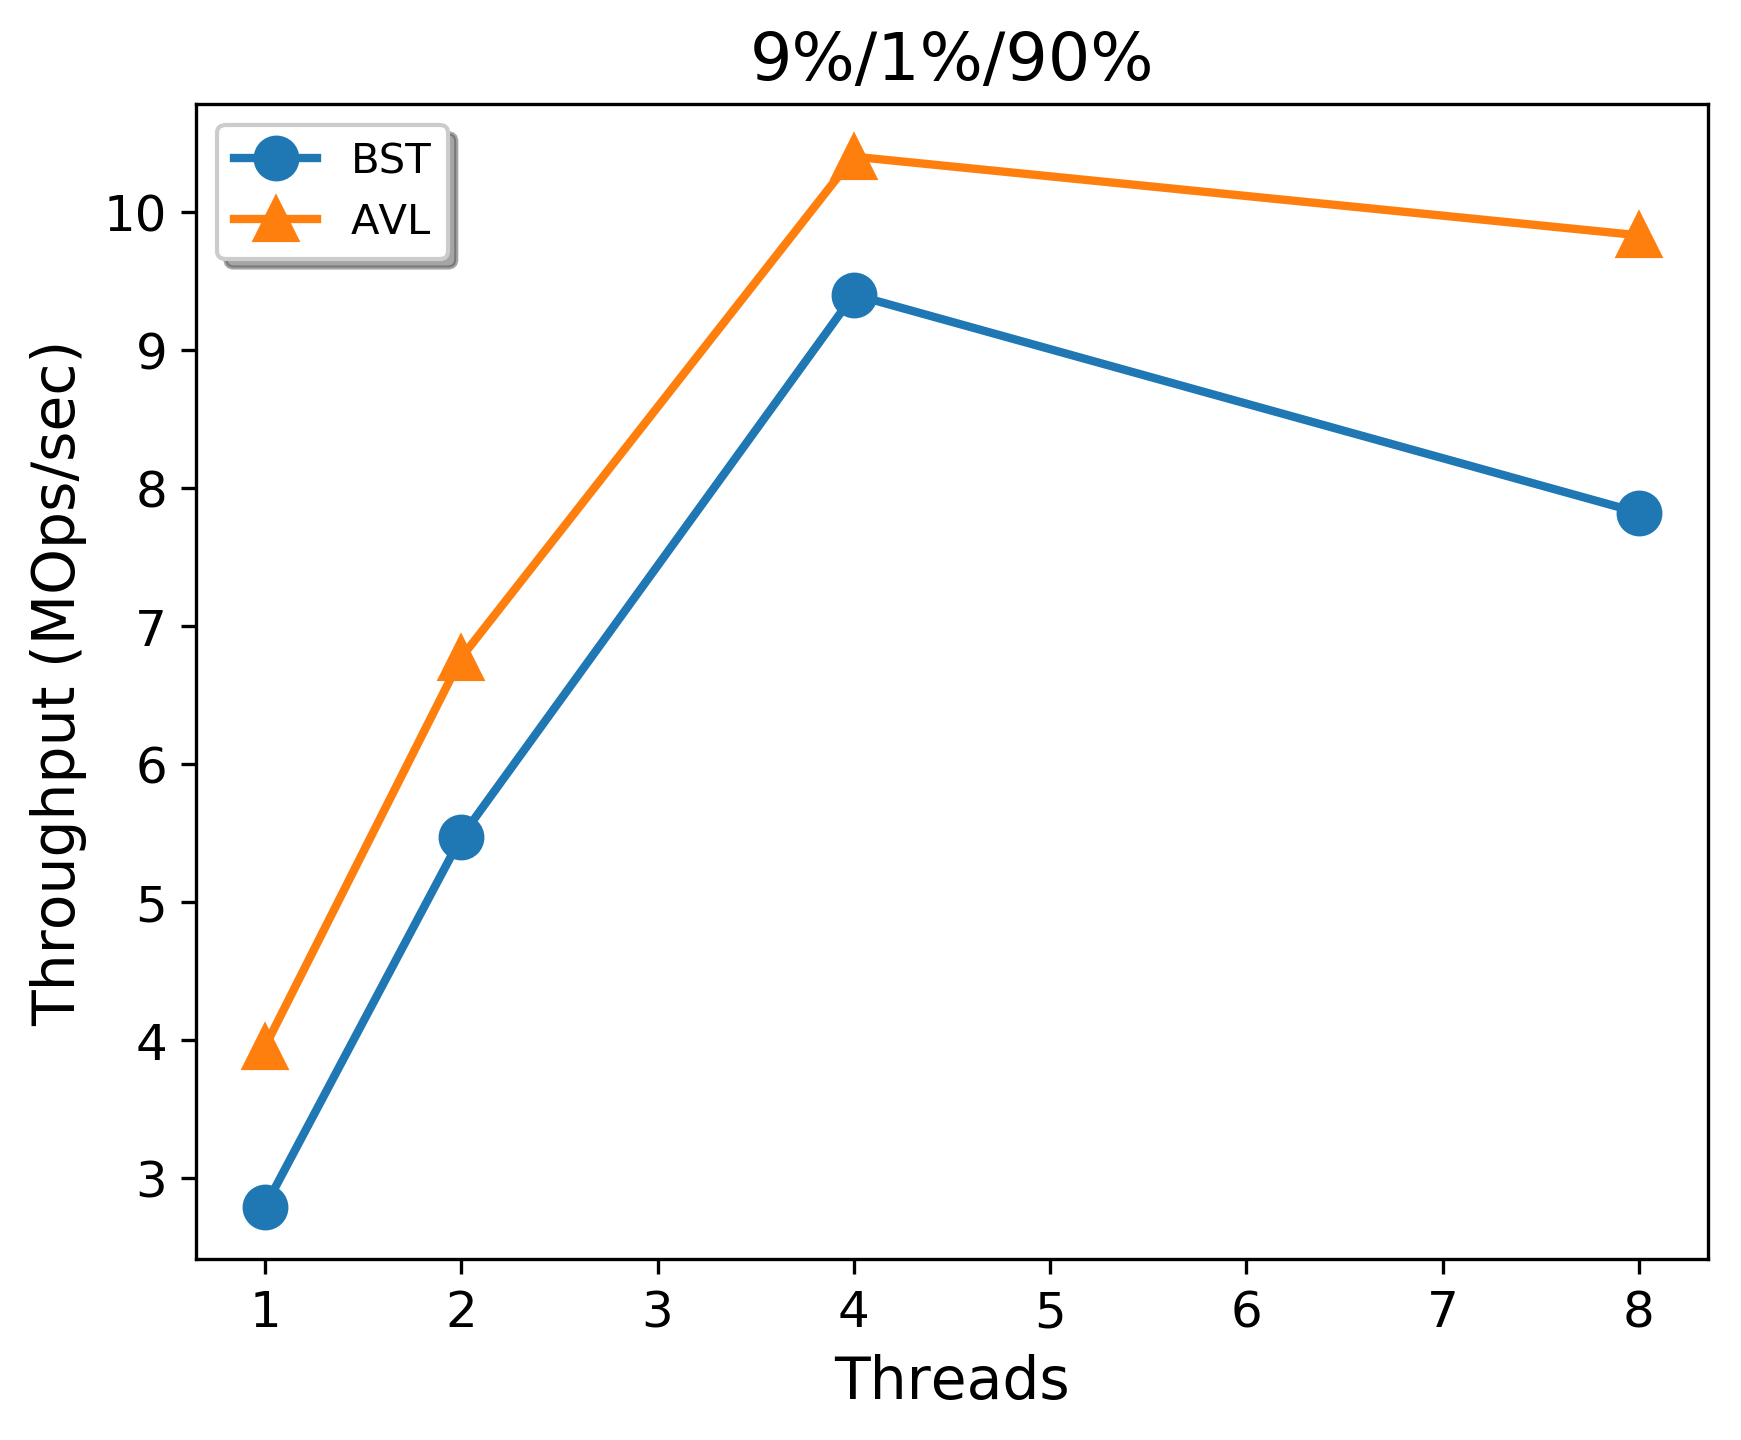
\includegraphics[width =1\linewidth]{figures/conc-9-1-90.png}}
 \subcaptionbox{STM}
 {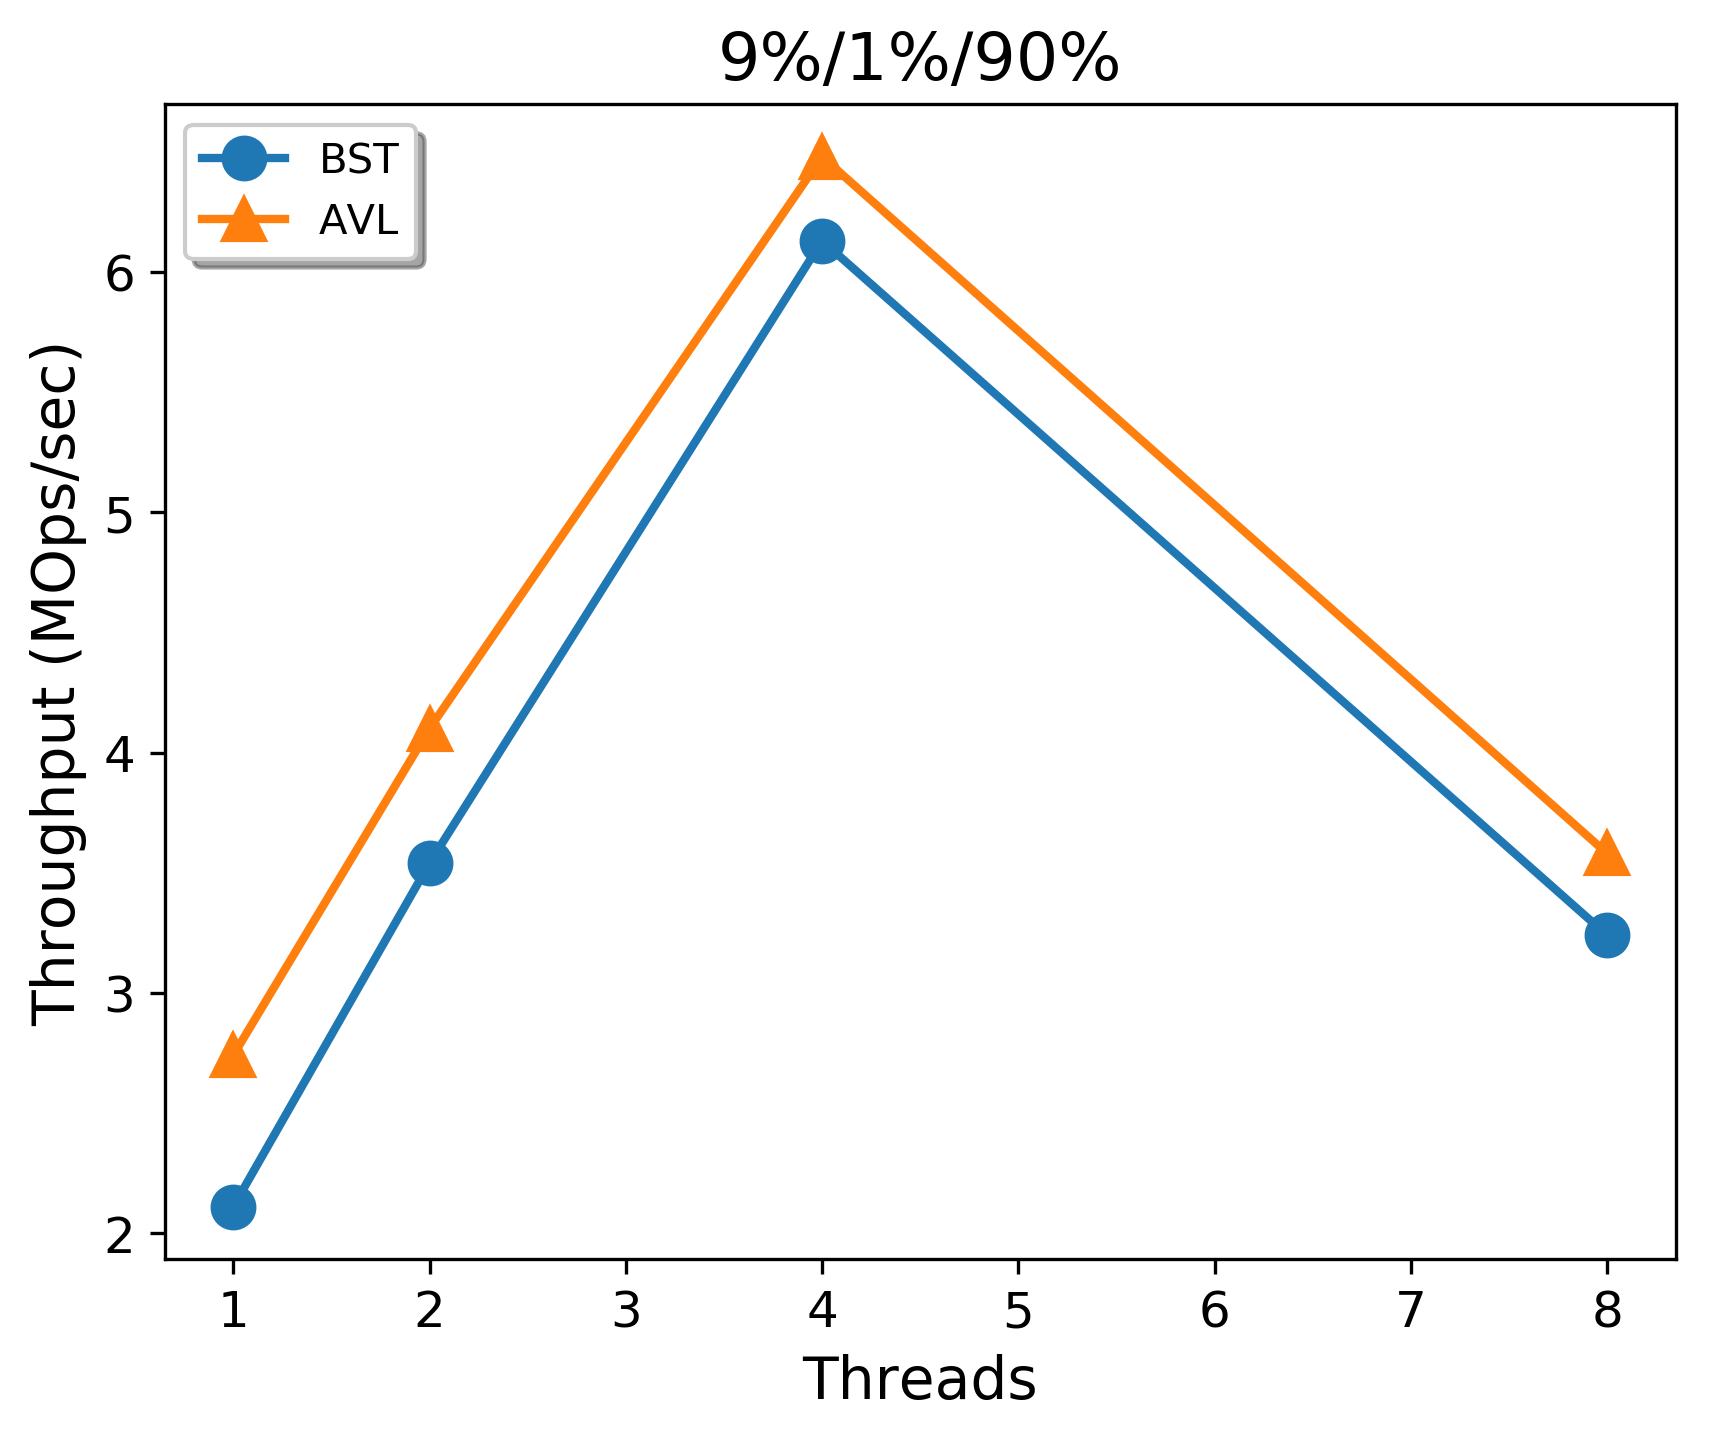
\includegraphics[width =1\linewidth]{figures/stm1-9-1-90.png}}
 \subcaptionbox{Modified STM}
 {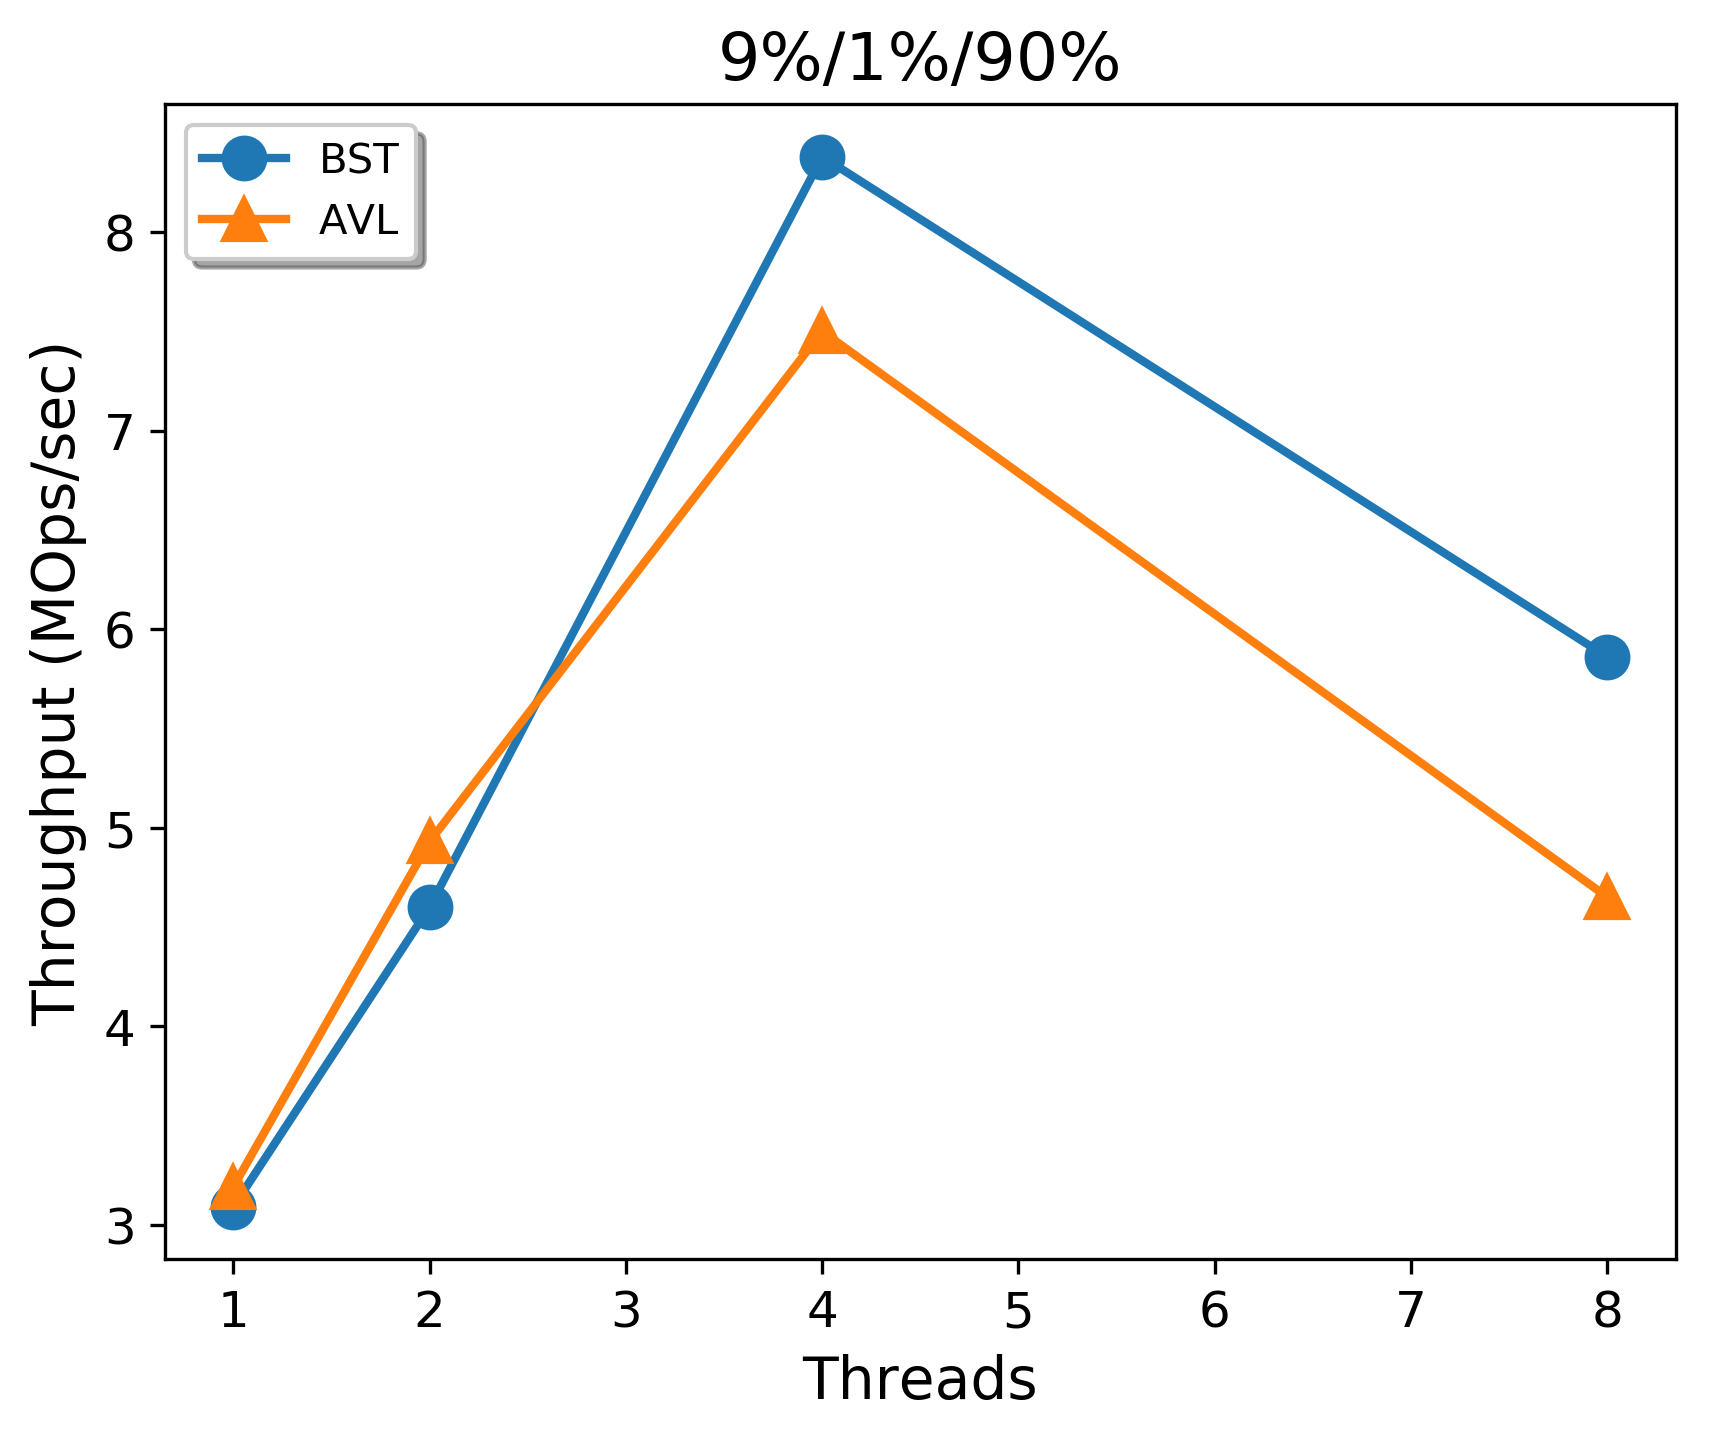
\includegraphics[width =1\linewidth]{figures/stm2-9-1-90.png}}
\end{minipage}%
\begin{minipage}{0.33\textwidth}
 \subcaptionbox{Locking}
 {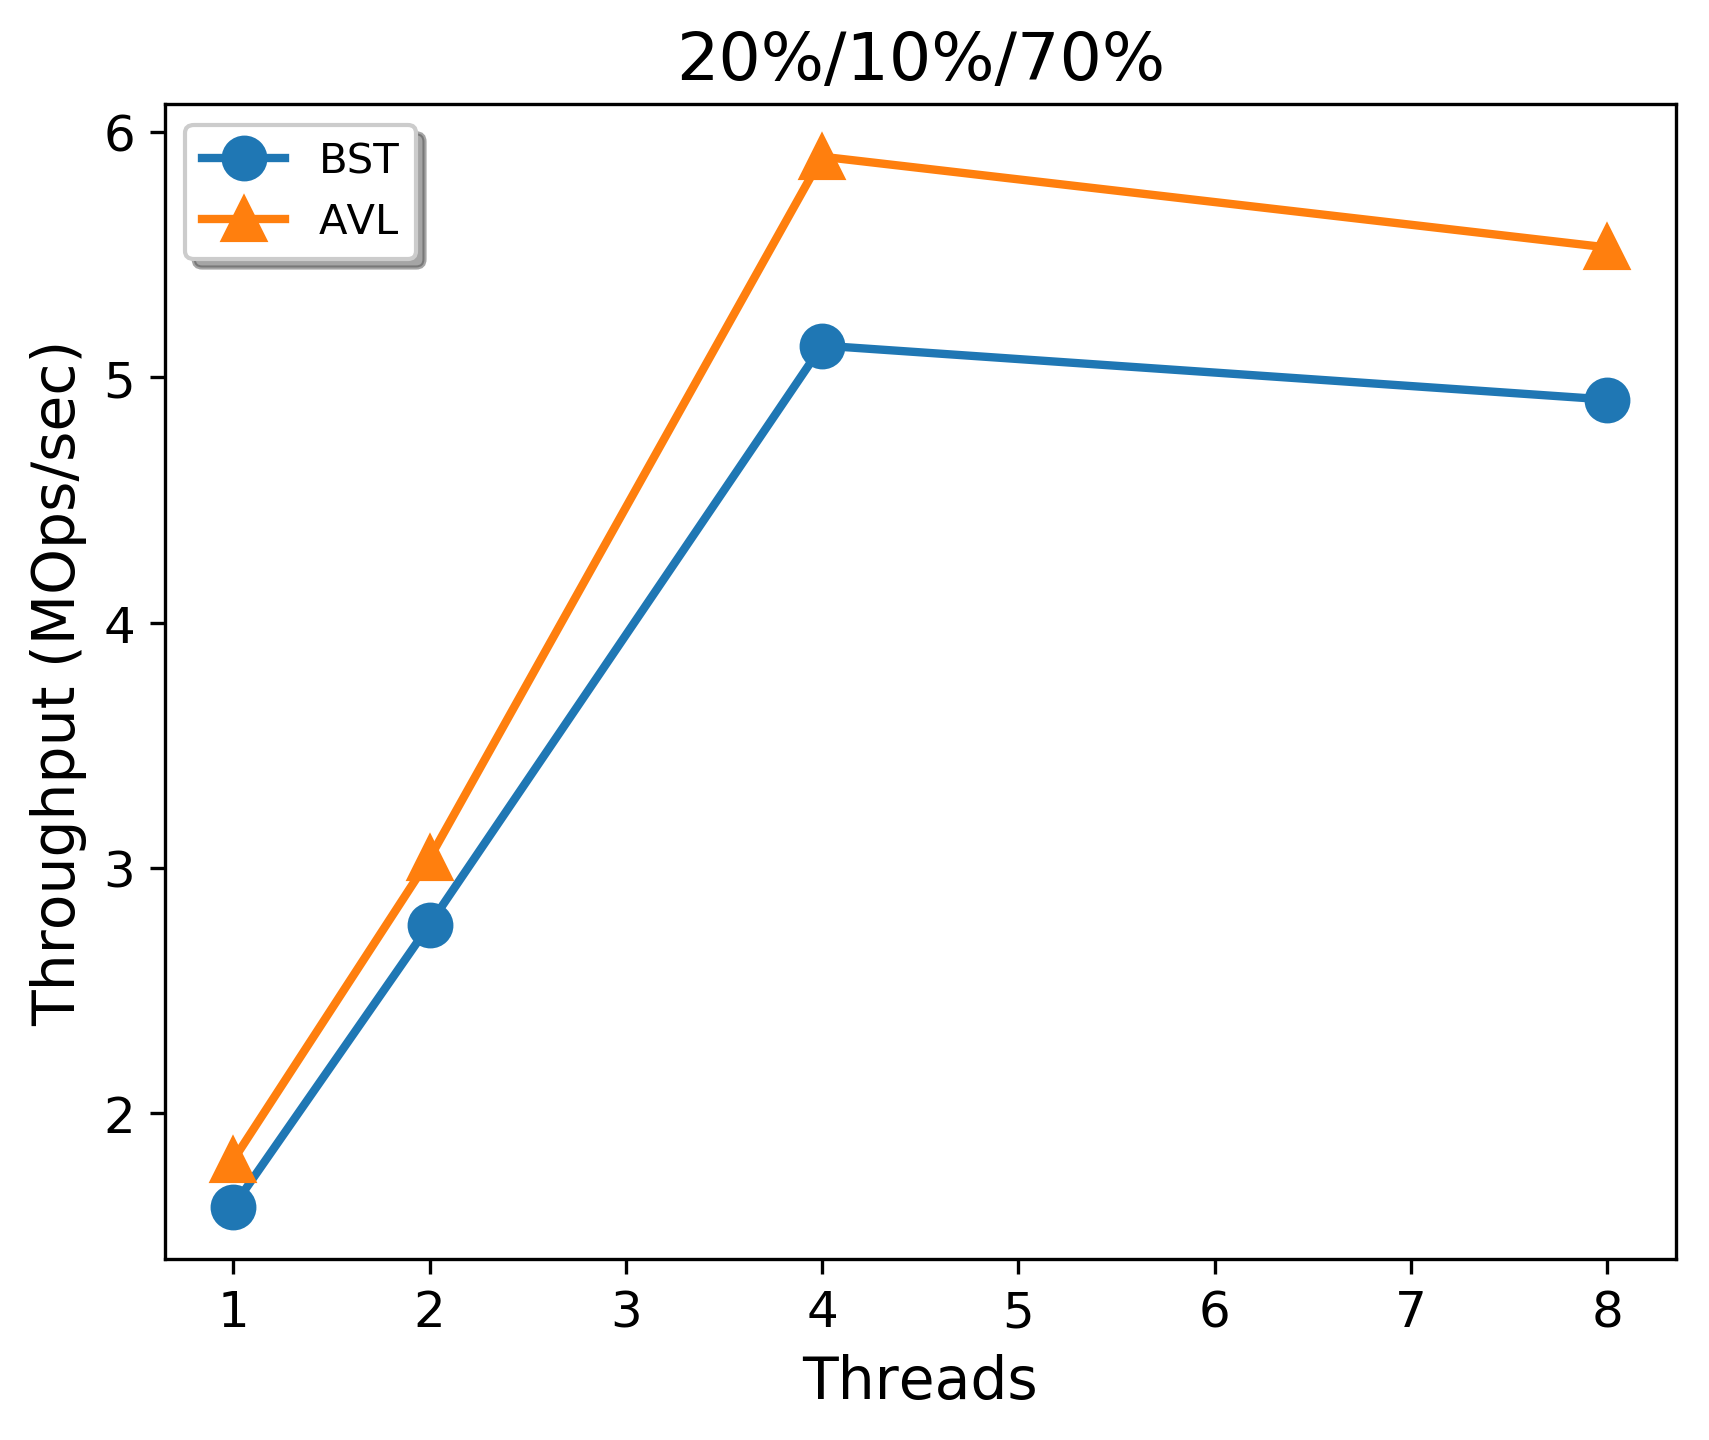
\includegraphics[width =1\linewidth]{figures/conc-20-10-70.png}}
 \subcaptionbox{STM}
 {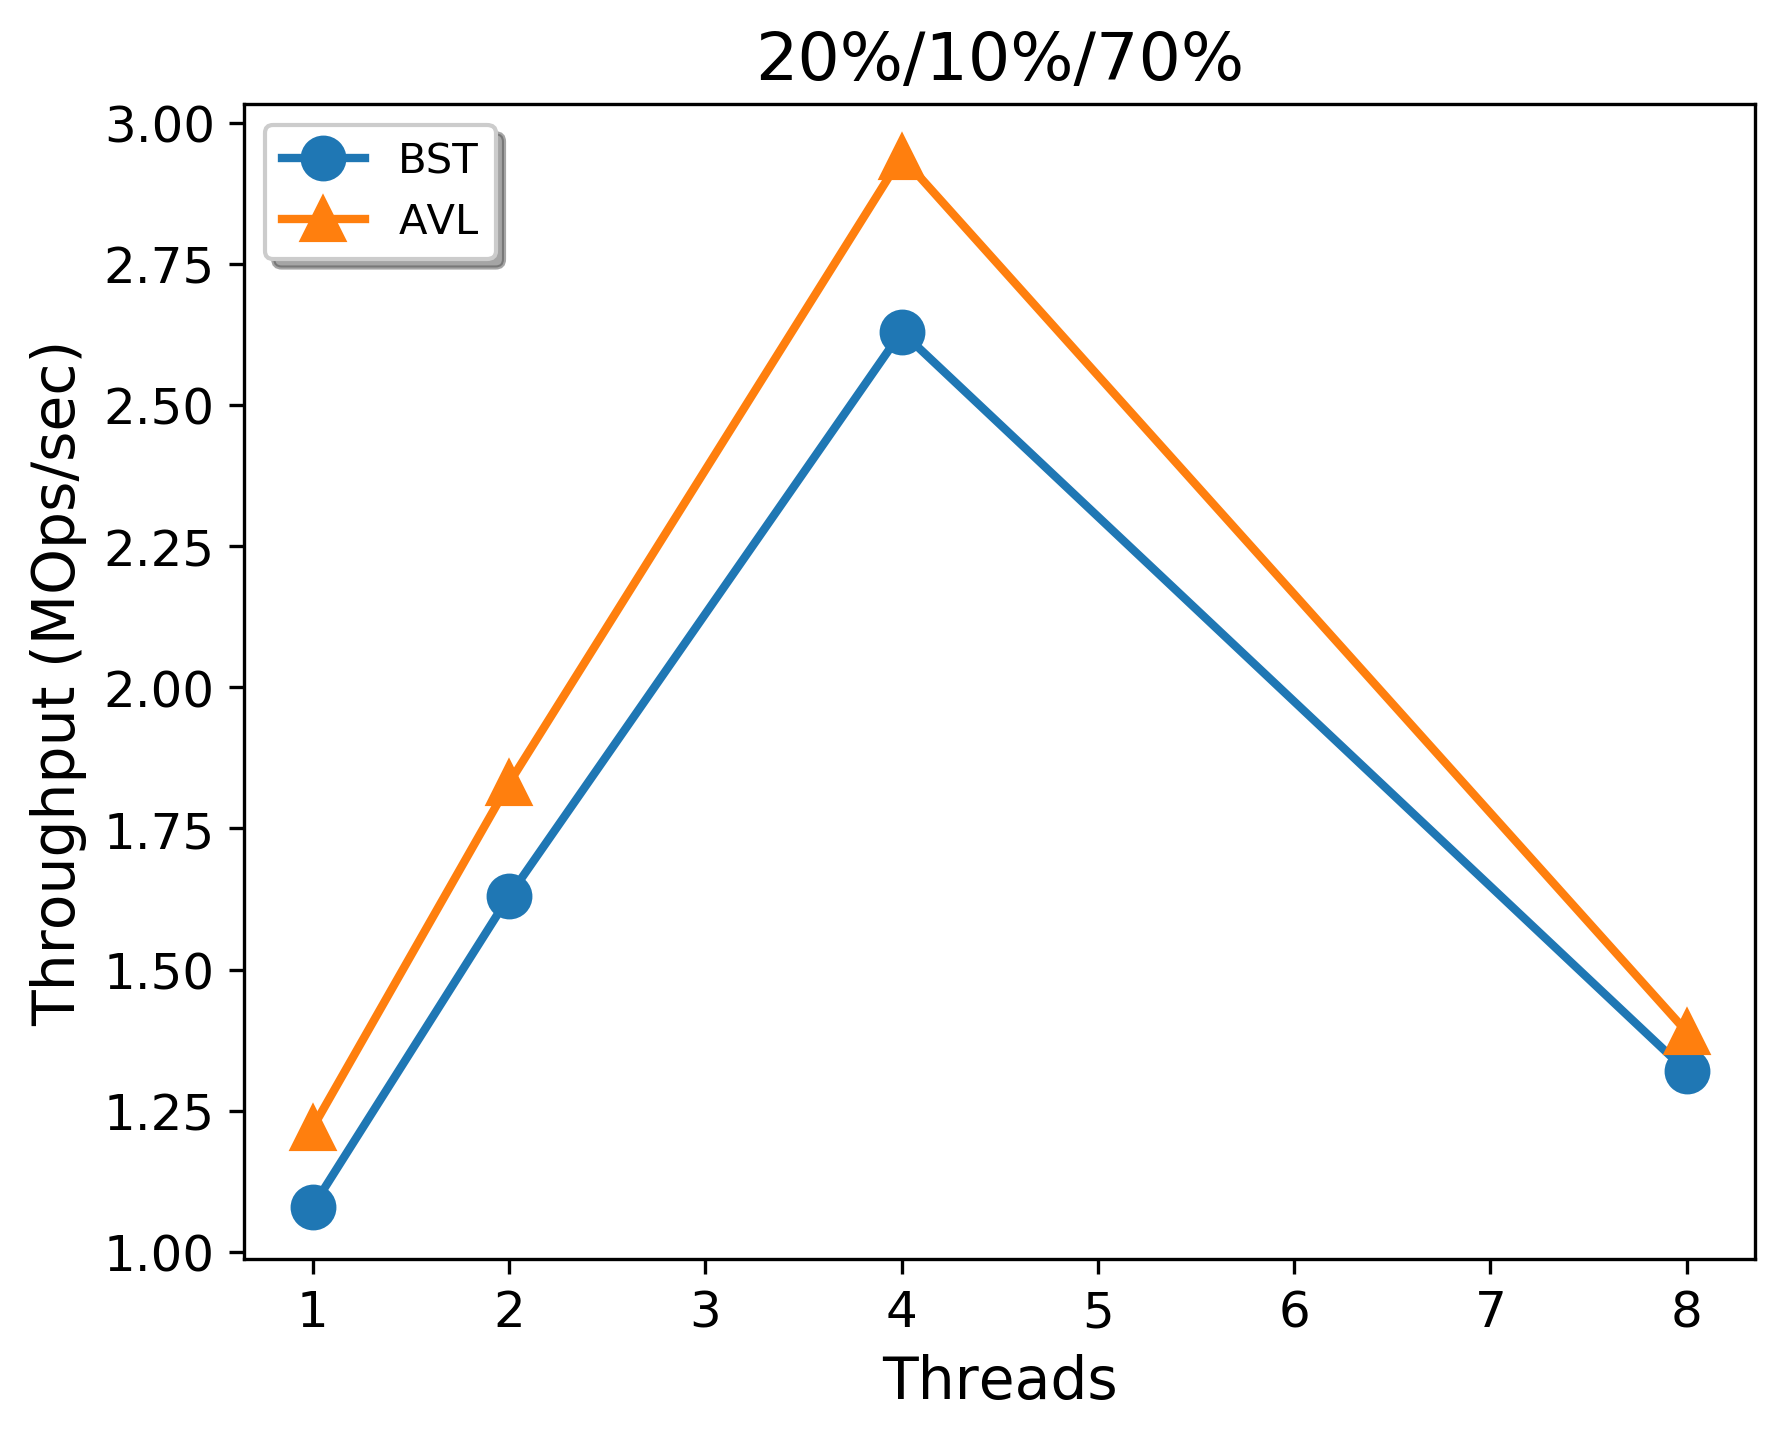
\includegraphics[width =1\linewidth]{figures/stm1-20-10-70.png}}
 \subcaptionbox{Modified STM}
 {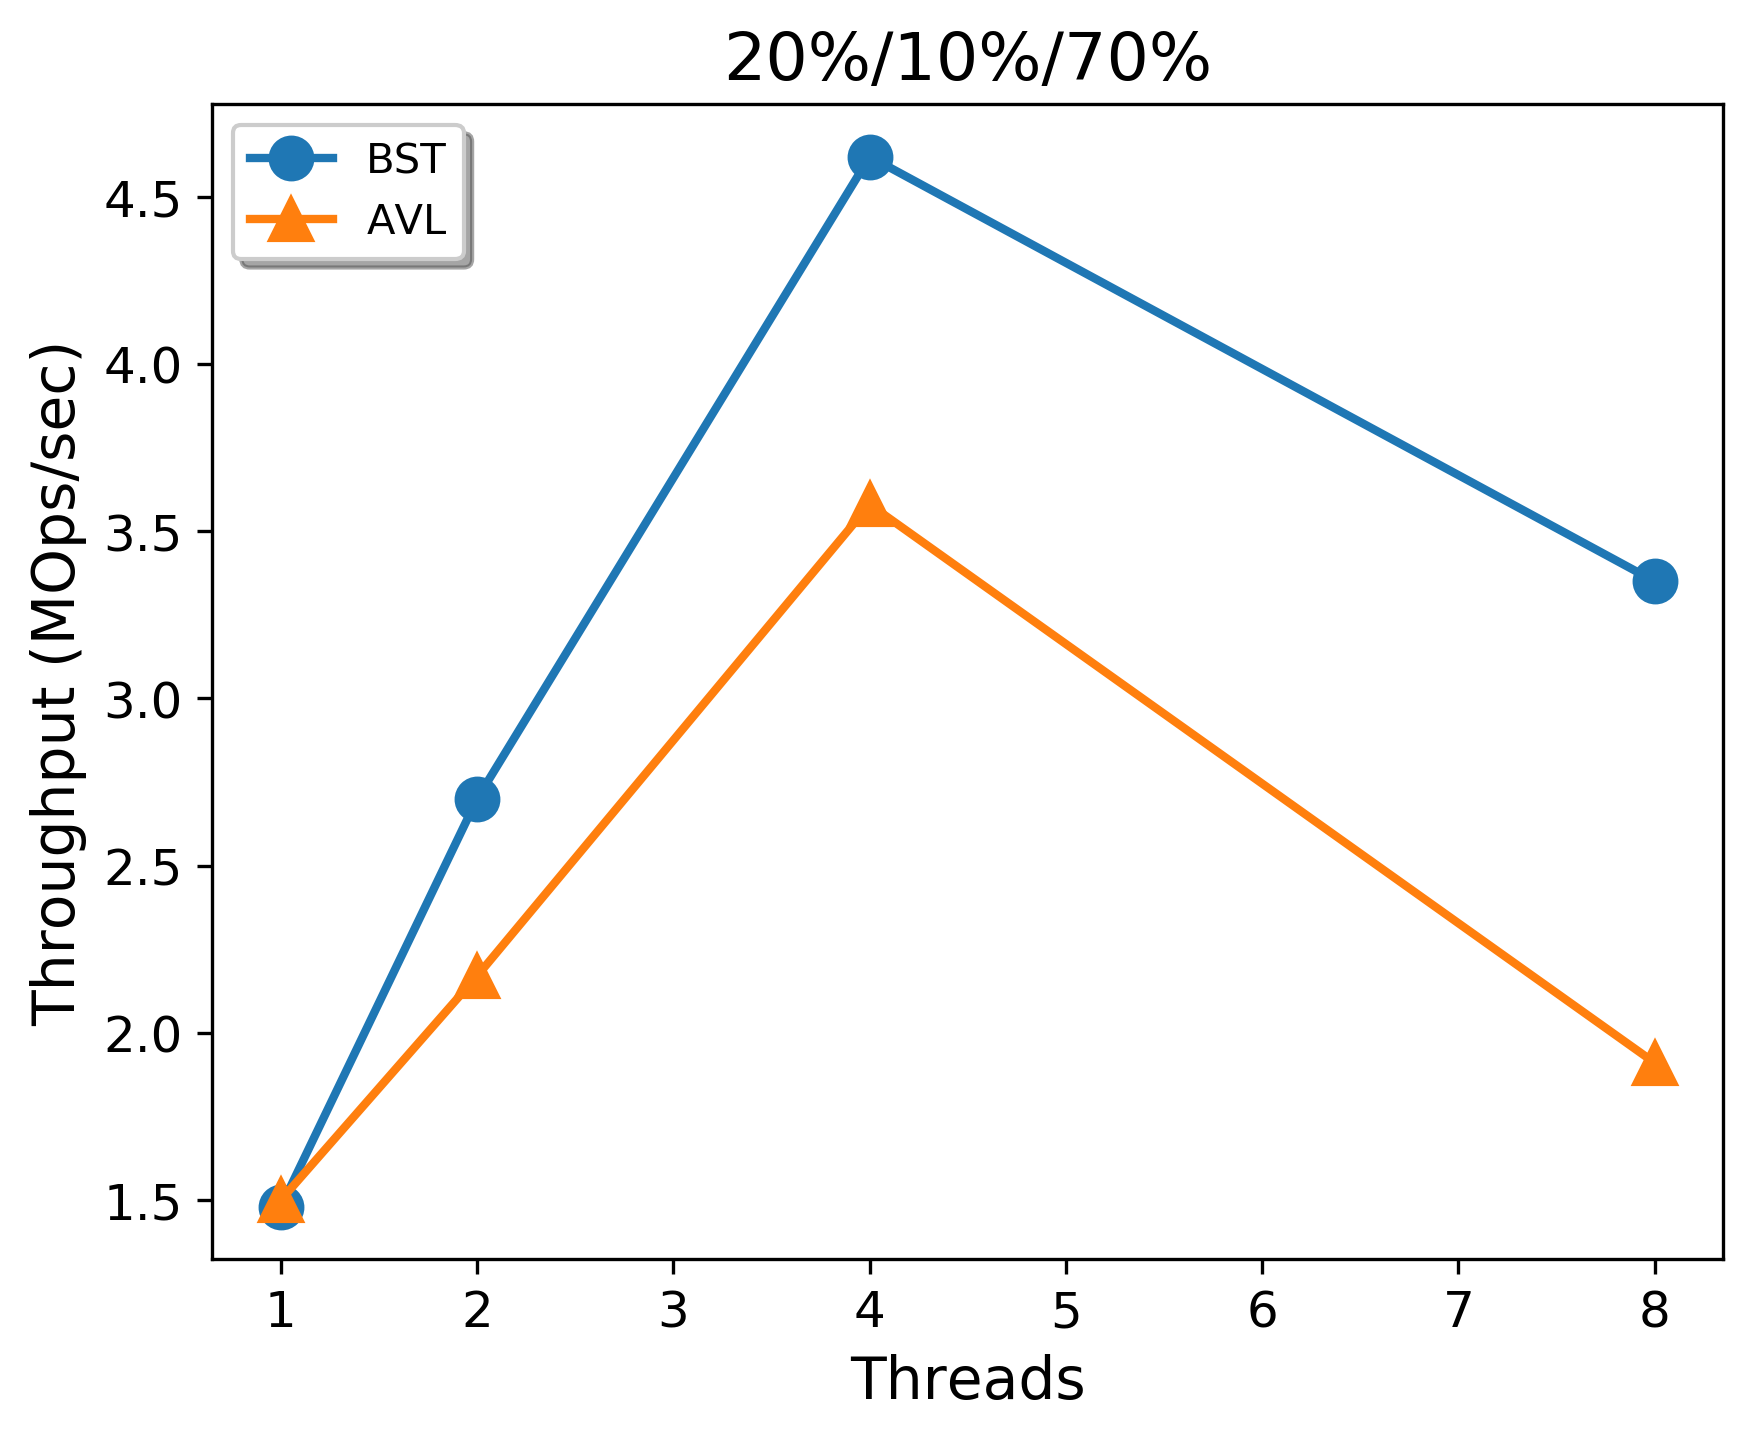
\includegraphics[width =1\linewidth]{figures/stm2-20-10-70.png}}
\end{minipage}
\begin{minipage}{0.33\textwidth}
 \subcaptionbox{Locking}
 {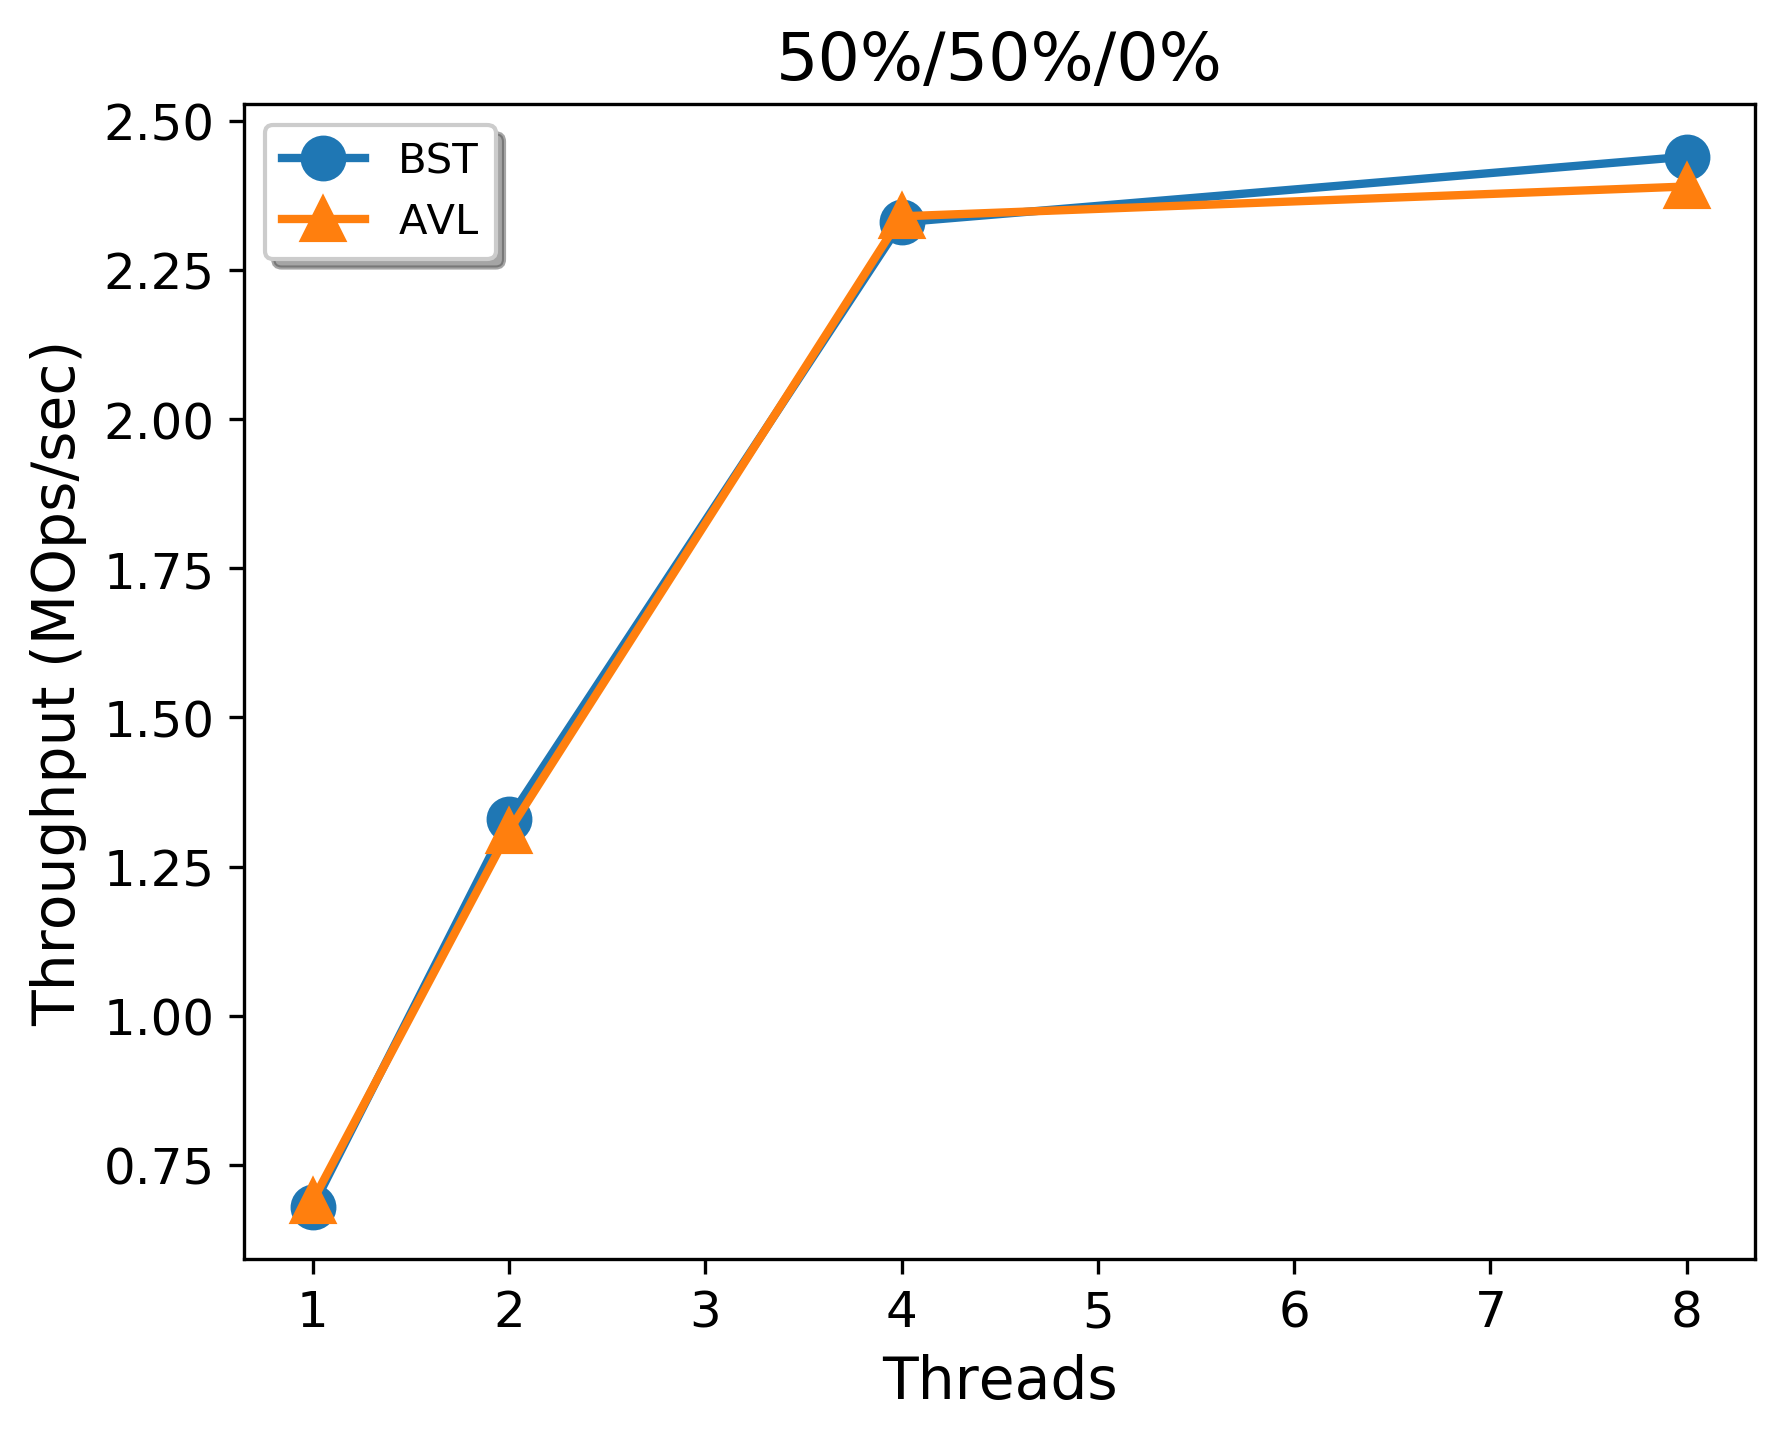
\includegraphics[width =1\linewidth]{figures/conc-50-50-0.png}}
 \subcaptionbox{STM}
 {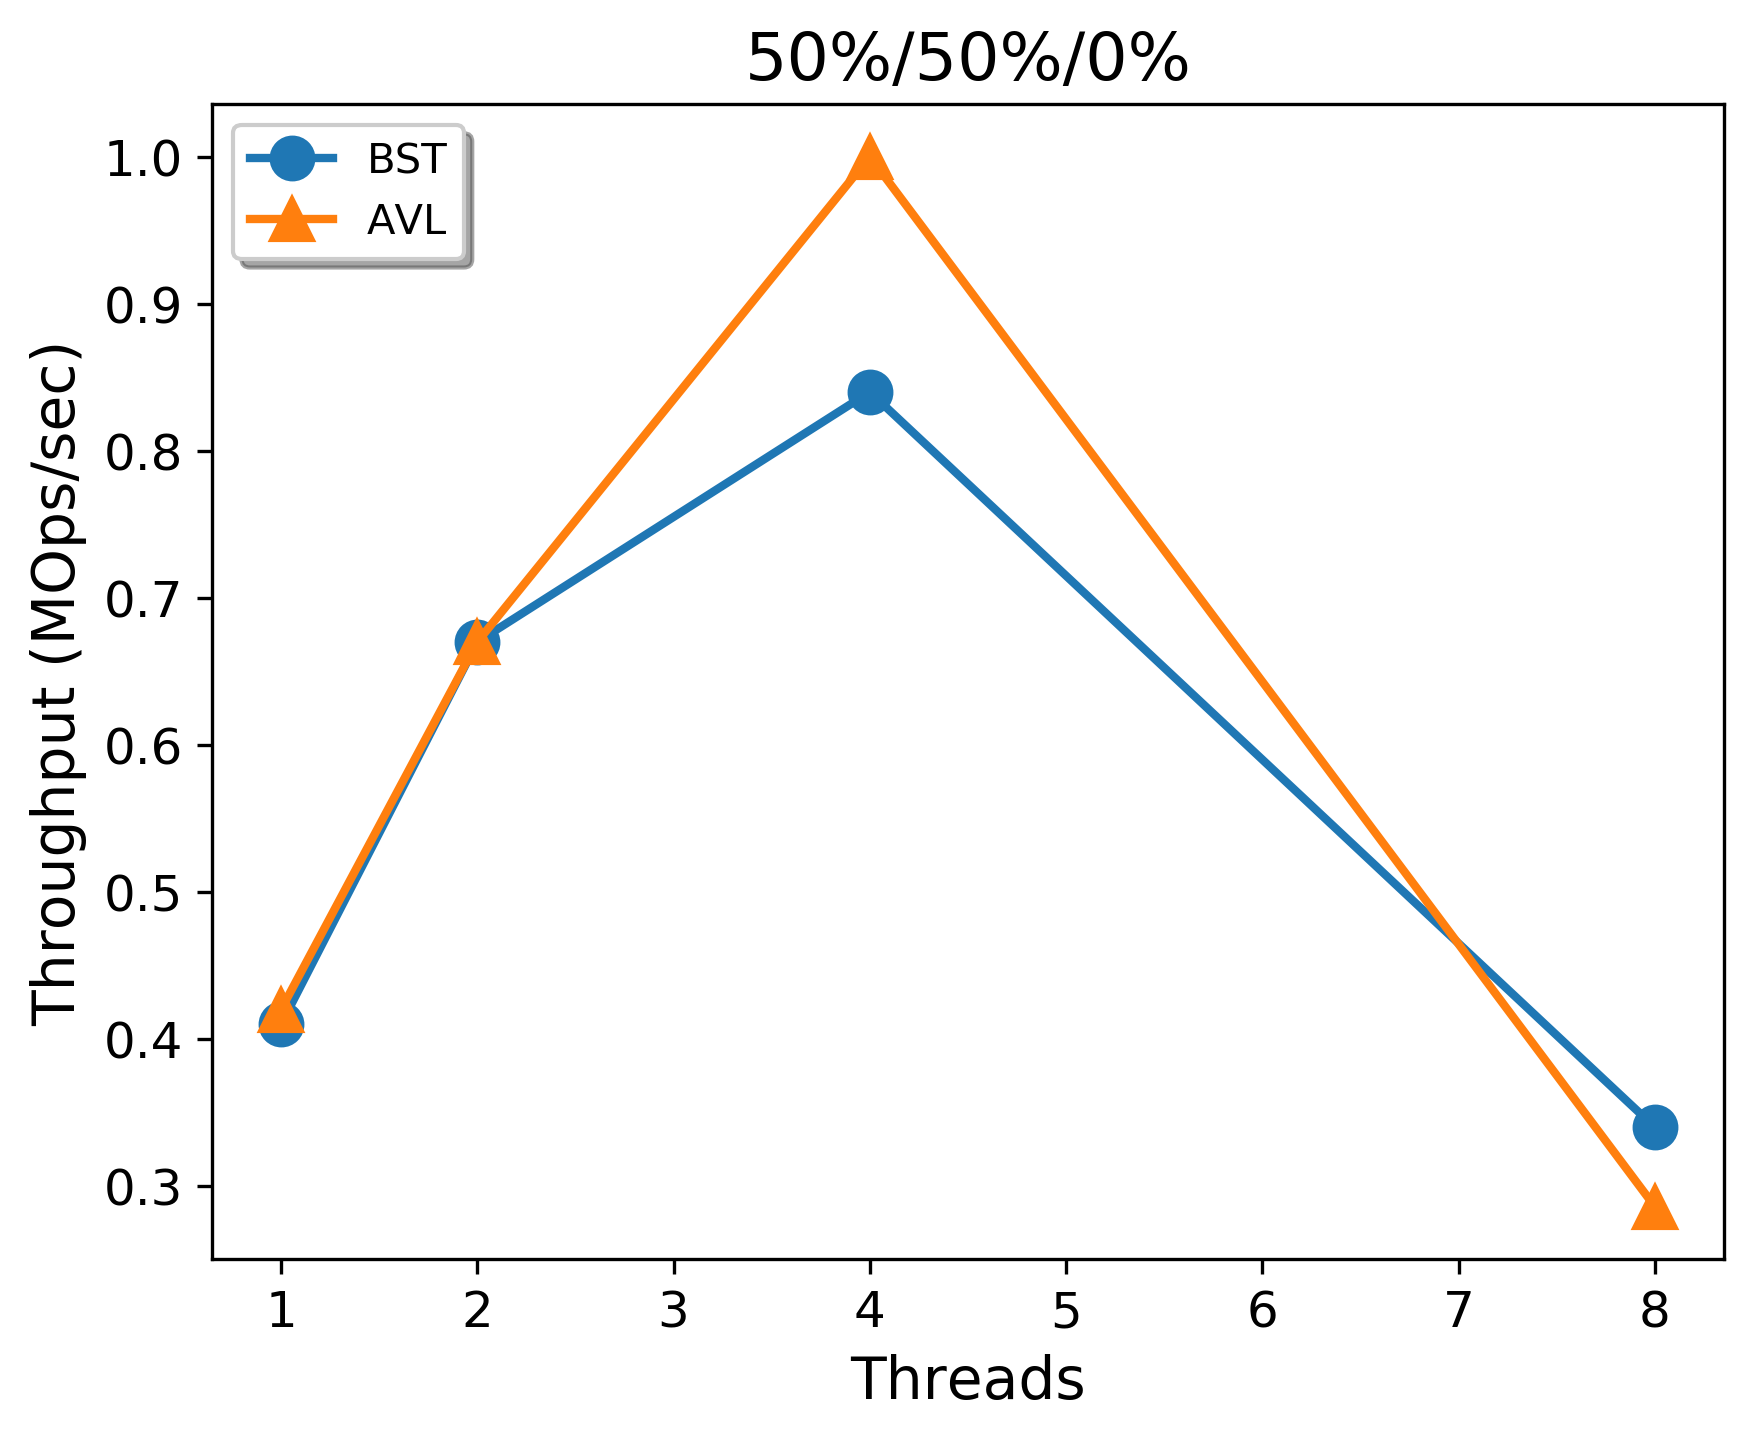
\includegraphics[width =1\linewidth]{figures/stm1-50-50-0.png}}
 \subcaptionbox{Modified STM}
 {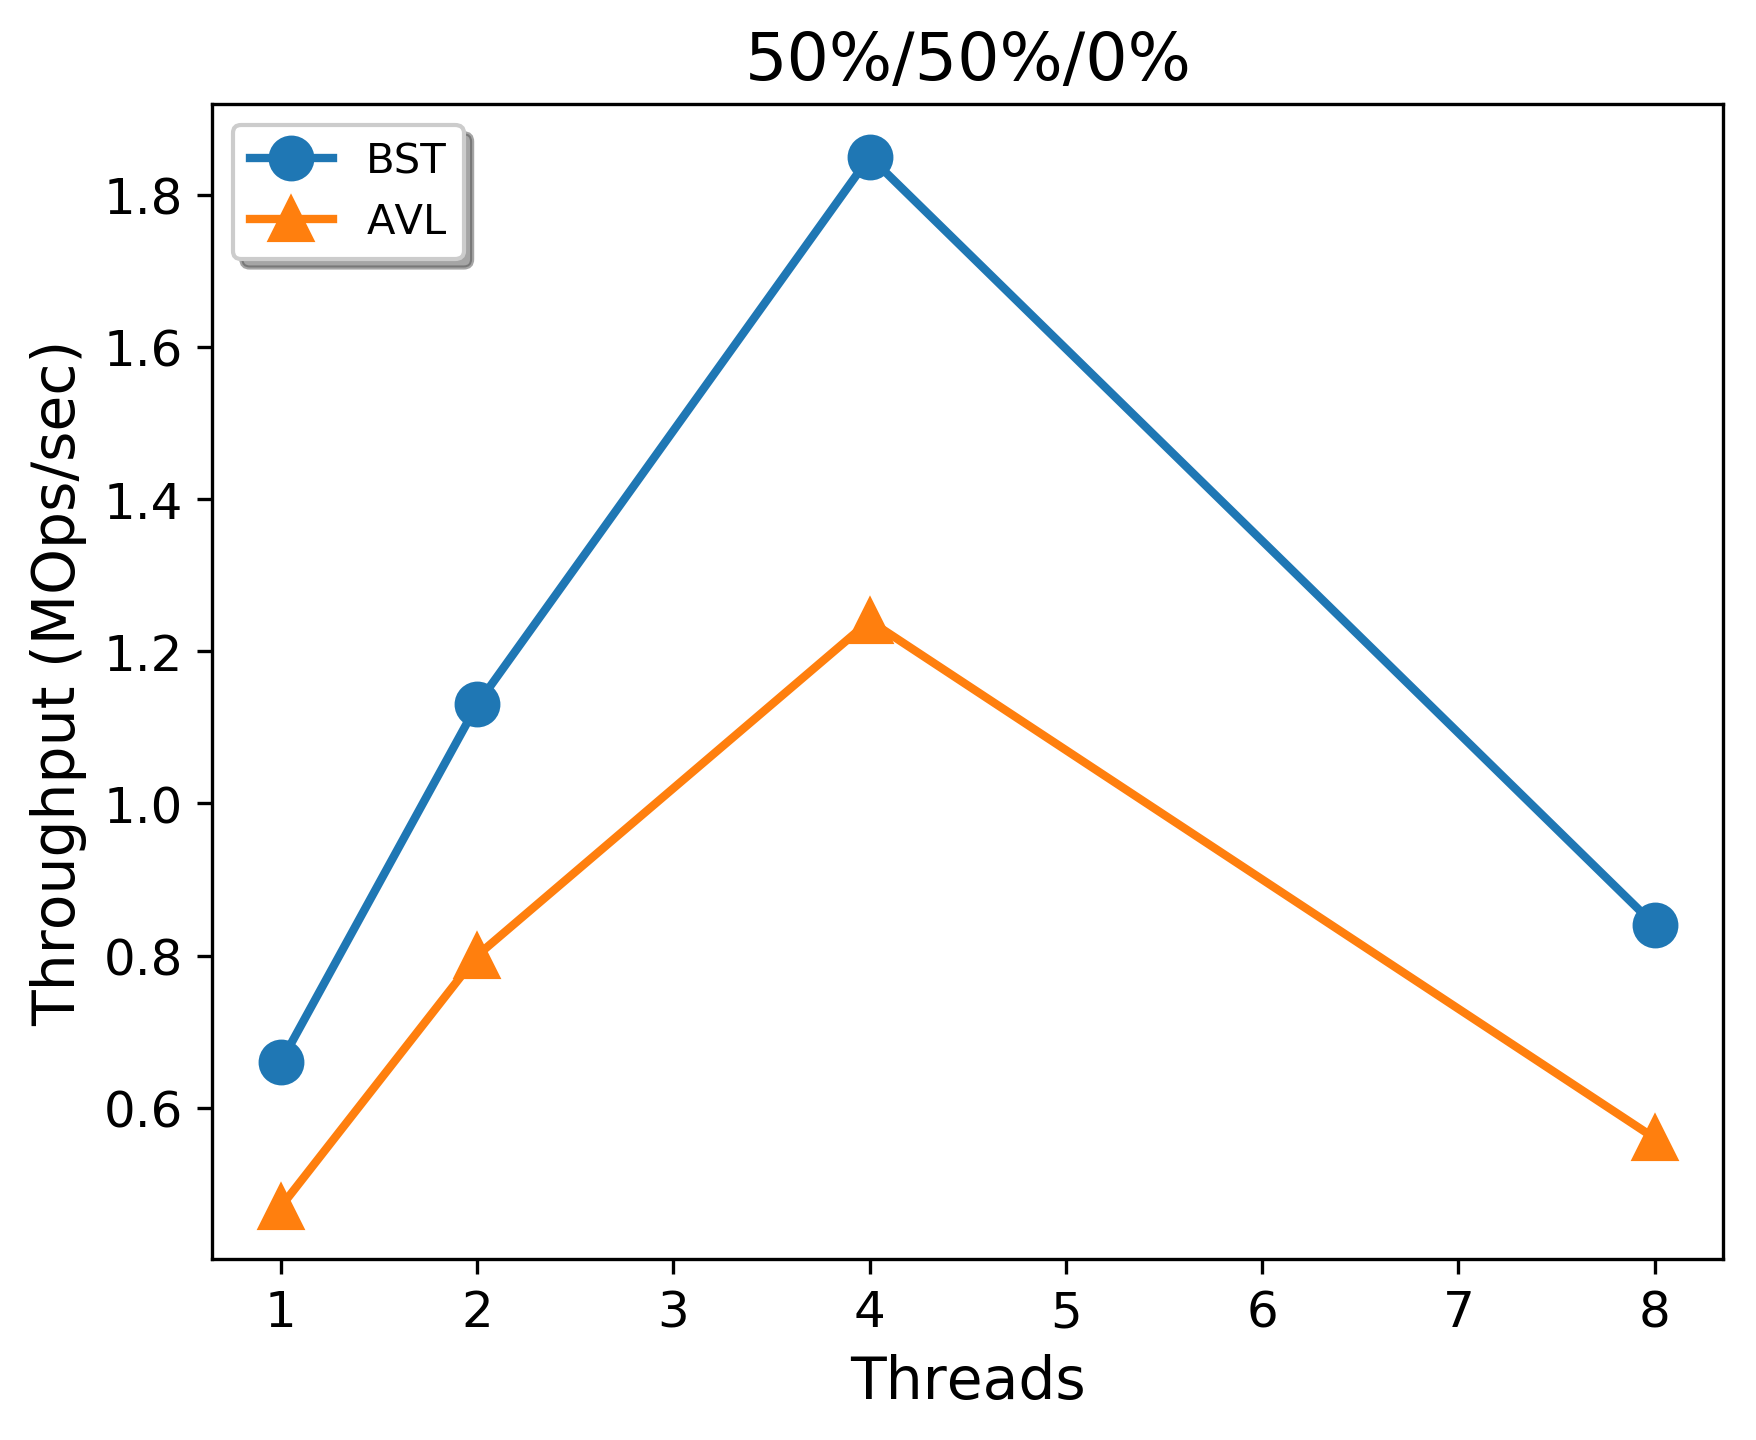
\includegraphics[width =1\linewidth]{figures/stm2-50-50-0.png}}
\end{minipage}
\label{fig:data}
\caption{The performance results of all tests with each of the three data structure implementations.}
\end{figure*}%

\section{Discussion}
\subsection{Analysis Summary}
The locking PaVT BST and AVL trees should to be highly scalable for the architecture that they were run on. Running the data structures on a larger number of cores could depict the true limitation for the data structure. The performance limitations became very obvious in the STM data structures. The performance would result in a sequential if not worse performance. However, the STM framework provided a relaxed programming effort for lock management as opposed to the locking requirements of the original implementation. The PaVT condition proved to provide a large amount of concurrency as seen in the $9\%/1\%/90$ tests. Due to the lock-free nature of the \textbf{contains} method, only a small atomic transaction for reading the snapshots was necessary which allowed for a high concurrent environment before improving the STM data structure. 

\subsection{Development Issues Encountered}
Providing synchronization in updating the snapshots proved to be a challenging aspect due to the few details provided by the author's. Their previous work with the logical ordering provided an initial starting point on how to maintain the snapshots. After contacting the authors, the algorithm became very simple to implement. The following difficulty that arose from synchronization came from the lock management of the removal method. There were two defining challenges with the locking protocol in \textbf{remove()}: (1) Managing locks that have already have been acquired. Although previously mentions in the details of \textbf{remove()}, there are some instances where two locks are needed that pertain to the same node (i.e., locking the successor's parent $p_s$ and $n$'s right child, $r$, which are the same node). The second difficulty came from preserving locking order upon releasing locks. This was addressed by providing Boolean to indicate if the lock needed to be locked (from a case of the first challange). This created code bloat which was solved by the STM implementations. The locking order became a problem during the rebalancing operations as the locking order changed with rotations. The design of the \textbf{rebalance} function was designed to address this problem to easily determine which locks would need to be unlocked first.

\begin{thebibliography}{00}
\bibitem{b1} D. Drachsler-Cohen, M. Vechev, and E. Yahav. 2018. Practical concurrent traversals in search trees. In Proceedings of the 23rd ACM SIGPLAN Symposium on Principles and Practice of Parallel Programming (PPoPP '18). ACM, New York, NY, USA, 207-218. DOI: https://doi.org/10.1145/3178487.3178503


\bibitem{b4} V. Luchangco, J. Maurer, M. Moir, H. Boehm, J. Gottschlich, M. Michael, T. Riegel, M. Scott, T. Shpeisman, M. Spear, M. Wong, "Transactional Memory Support for C++",[online document], 2013. Available: JtC1/SC22 subcommittee, http://www.open-std.org [Accessed: November 29, 2018]

\bibitem{bron}
Bronson, N. G., Casper, J., Chafi, H., Olukotu, K. (2014). A practical concurrent binary search tree. In PPoPP'14.

\bibitem{crain-cont}
Crain, T., Gramoli, V., Raynal, MA Contention-Friendly Binary Search Tree. In Euro-Par '13.

\bibitem{crain-stm}
Crain, T., Gramoli, V., Raynal, M. (2011) A transaction-friendly binary search tree.  [Research Report] PI-1984, pp.21. <inria-00618995v1>

\bibitem{draschler-lo}
Draschler, D., Vechev, M., Yahav, E. (2014) Practical Concurrent Binary Search Trees via Logical Ordering. In PPoPP'14.
\end{thebibliography}

\end{document}
